% $Id: thesis.tex,v 1.60 2010/04/13 11:12:30 dvd Exp $

\documentclass[oneside]{report}

\usepackage{algorithm,algorithmic}
\usepackage{url}
\usepackage{setspace,geometry}
\usepackage{framed}
\usepackage{amsfonts,amsmath,amsthm}
\usepackage{graphicx}

\usepackage{tikz}
\usetikzlibrary{positioning}
\usetikzlibrary{shapes.geometric}
\usetikzlibrary{shapes.symbols}
\usetikzlibrary{shadows}
\usetikzlibrary{arrows}

\geometry{bindingoffset=0.4in,margin=1.2in}
\onehalfspacing
\doublespacing

% $Id: defs.tex,v 1.3 2009/07/24 11:21:04 dvd Exp $ 
\newcommand {\mean} {\ensuremath {\mathop{\mathrm{mean}}}}
\newcommand {\median} {\ensuremath {\mathop{\mathrm{median}}}}
\newcommand {\N} {\ensuremath {\mathcal{N}}}
\newcommand {\IE} {\ensuremath {\mathbb{E}}}
\newcommand {\cov} {\ensuremath {\mathop{\mathrm{cov}}}}
\newcommand {\BEL} {\ensuremath {\mathop{\mathrm{BEL}}}}

\newtheorem{thm}{Theorem}
\newtheorem*{dfn}{Definition}
\newtheorem{lemma}{Lemma}
\newtheorem{crl}[thm]{Corollary}

\newcommand{\OPEN} {{\textsc{Open}}}
\newcommand{\CLOSED} {{\textsc{Closed}}}
\newcommand{\astar} {\ensuremath{A^\ast}}
\newcommand{\lazyastar} {\ensuremath{LA^\ast}}
\newcommand{\rationallazyastar} {\ensuremath{RLA^\ast}}



\title {Rational Metareasoning in Problem-Solving~Search}

\author {David Tolpin}

\begin{document}

\begin{titlepage}
\begin{center}
{\large Ben-Gurion University of the Negev
\\
Kreitman School for Advanced Graduate Studies}
\vspace{1in}

{\bf\LARGE Rational~Metareasoning in Problem-Solving~Search}
\vspace{1in}

{\large PhD Thesis Proposal
\\
\vspace{1in}

by David Tolpin
\\
Under the supervision of Professor Solomon Eyal Shimony
\\
\vfill

\today}

\vspace{1in}
%Author's Signature: \rule{10em}{1pt}
%\\
%Advisor's Signature: \rule{10em}{1pt}
%\\
%Chairman's Signature: \rule{10em}{1pt}

\end{center}
\end{titlepage}

\pagenumbering{roman}

\setcounter{page}{1}
\pagenumbering{roman}

An important class of Artificial Intelligence problems is
problem-solving search. In problem-solving search, a single agent acts
in a neutral environment to reach the goal. Many problems, such as
routing and path-finding problems, finite-domain constraint
satisfaction, function optimization, fit within the problem-solving
search abstraction. General search algorithms capable of solving large
sets of search problems are well known. Algorithm performance can be
significantly improved by tuning the algorithm to a particular problem
domain; however, such fine-tuned algorithms exhibit good performance
only on small sets of search problems, and the effort invested in the
algorithm design cannot be reused in other problem domains.

Specialized versions of general search algorithms are often created by
combination and selective application of search  heuristics.
A human expert decides which heuristics to use with the
problem domain, and specifies how the search algorithm should apply
the heuristics to solve a particular problem instance. A search
algorithm that rationally selects and applies heuristics would decrease
the need for the costly human expertise. Principles of rational
metareasoning can be used to design rational
search agents.

Some rational search algorithms were designed and shown to compare to
or even outperform manually tuned algorithms. However, wide adoption
of rational metareasoning algorithms for problem solving search is
hindered both by theoretical difficulties and by lack of problem
domain specific case studies. This research aims at lifting some of
the theoretical difficulties in application of the rational
methodology. In particular, the problem of efficiency estimating
the value of information of computational actions is considered. In
addition, this research proposes rational metareasoning versions of
algorithms for applications of problem-solving search in the areas of
parameter tuning, constraint satisfaction, canadian traveller problem,
and Bayesian network structure learning.


\setcounter{tocdepth}{5}
\tableofcontents
%\listoffigures
%\listoftables

\newpage
\setcounter{page}{1}
\pagenumbering{arabic}

\chapter{Introduction}
\label{ch:intro}
A common approach in Artificial intelligence (AI)
solves computational problems by designing {\em agents}. Agents
act in an environment, exploring and possibly modifying the
environment in order to reach the {\em goal}: a solution of the
problem. Agent behavior is determined by the {\em agent function} that
maps the agent's knowledge about the environment to actions. AI
classifies problems according to the number of agents, the type of
interaction among the agents and between the agents and the
environment, as well as by the {\em problem domain}---properties of
the environment which help design efficient problem-specific agents.

A simple yet large class of problems is {\em problem-solving
  search}. In problem-solving search, a single agent acts in a neutral
environment to reach the goal. Many problems, such as routing and
path-finding problems, finite-domain constraint satisfaction, function
optimization, fit within the problem-solving search abstraction. The
problem-solving search agent's behavior is described by a {\em search
  algorithm}. The same search algorithms can be used to solve
different search problems, but a general search algorithm often
requires adaptation to solve a particular problem efficiently.

Computer scientists approach problem-solving search in two ways. On
the one hand, general search algorithms capable of solving large sets
of search problems are designed, such as A* search for path-finding
problems, or the Maintaing Arc Consistency (MAC) algorithm for
finite-domain constraint satisfaction \cite{Russell.aima}. Theoretical
performance bounds can often be proved for these algorithms, and the
same algorithm can efficiently solve many problem instances with
little or no adaptation. On the other hand, the algorithm performance
can be significantly improved by tuning the algorithm to a particular
problem domain. For example, specialized algorithms for task
scheduling outperform general constraint satisfaction algorithms by
orders of magnitude \cite{Wolf.scheduling}. However, such fine-tuned
algorithms exhibit good performance only on small sets of search
problems, and the effort invested in the algorithm design cannot be
reused in other problem domains.

Specialized versions of general search algorithms are often created by
combination and selective application of {\em search
  heuristics}---domain-specific modifications or extensions of search
algorithms. A human expert decides which heuristics to use with the
problem domain, and specifies how the search algorithm should apply
the heuristics to solve a particular problem instance. A search
algorithm that rationally select and applies heuristics would decrease
the need for the costly human expertise.

The principles of rational metareasoning \cite{Russell.right} can be
used to design rational search agents. A rational agent deliberates
before acting. The deliberation is composed of {\em computational
  actions}. The purpose of the deliberation is to select the best {\em
  base-level action}. A base-level action affects the state of the
search algorithm looking for a solution of a problem instance, for
example, by a exploring the search space, or pruning a part of the
search that does not contain a solution. Computational actions are
selected according to their net value of information, the difference
between the expected benefit and the cost of the action, and the agent
deliberates only if there is a computational action with positive
value of information.

Some rational search algorithms were designed and shown to compare to
or even outperform manually tuned algorithms
\cite{Russell.right}. However, wide adoption of rational metareasoning
algorithms for problem solving search is hindered both by theoretical
difficulties and by lack of problem domain specific case studies. This
research aims at lifting some of the theoretical difficulties in
application of the rational methodology. In particular, the problem of
efficiency of estimating the value of information of computational
actions is considered. In addition, this research proposes rational
metareasoning extensions for several search algorithms, and
theoretically and empirically analyses the gain in performance due to
the extensions.

The rest of the thesis is organized as follows. Chapter~\ref{ch:bg}
provides the necessary background information about the rational
metareasoning approach as well as about search problems and
algorithms. Chapter~\ref{ch:ramesrch} describes application of the
rational metareasoning approach to search problems and discusses
difficulties arising in design of search algorithms based on the
approach. Chapter~\ref{ch:raticomp}, based
on \cite{TolpinShimony.raticomp}, introduces rational computation of
value of information---an important issue in design of efficient
search algorithms based on rational metareasoning. Case studies of the
rational metareasoning approach in several search problems are
presented and evaluated in Chapter~\ref{ch:case-studies} (based
on~\cite{TolpinShimony.csp,TolpinShimony.mcts,HayRussellTolpinShimony.selecting,TolpinEtAl.rla}).
Chapter~\ref{ch:summary} concludes this thesis with a discussion of
achieved results and further research directions.


\chapter{Background}
\label{ch:bg}

\section{Rational Metareasoning}
\label{sec:ratimeta}
While ideally programs, or agents, should {\em act rationally}
\cite{Russell.aima}, absolute rationality is not feasible. The
computational power of the agent approaching the problem must be taken
into account. Rational metareasoning \cite{Russell.right} is an
approach to building {\em bounded optimal} agents, agents which find a
solution that is optimal given their computational resources
\cite{Horvitz.reasoningabout}. The approach describes a method of
choosing {\em meta-level actions} and is based on notions of {\em
value of information} and {\em time cost}.

\subsection{Meta-level Actions}

The rational meta-reasoning framework aims at optimal
decision-making w.r.t. which computational operator should be applied
at every point in the search. In rational meta-reasoning, one can
define a meta-level decision problem over states of the belief space
with computational operators as meta-level actions, as a problem of
sequential decision-making under uncertainty. This meta-level problem
can be formalized as a (belief state) meta-level Markov decision
process (MDP) defined by a tuple $(Q, M, \pi, R)$ as follows:
\begin{itemize}
\item $Q$ is the state space. Each state $Q_i \in Q$ includes all
current knowledge about the search graph. For example, in a
single-agent search problem a state is comprised of the known part of
the search graph, including all available heuristic estimates of nodes
of this graph. 

For every meta-level state $Q_i$ there is a
corresponding base-level action $A_i \in A$, which \textit{appears to
be the best action} given $Q_i$. \chg{For example, in a best-first
search algorithm (Section \ref{sec:bg-best-first-search}) 
a base-level action is expanding a node in the fringe.}

\item $M$ is the set of state transitions. The transitions---the
meta-level actions $M_j \in M$---are all the potential computational
operators that are applicable to a state $Q_i$, such as calculating an
heuristic for a given node. The transition probabilities $\pi$ are
defined by the distributions over new knowledge that may be revealed
by applying each of the potential computational operators.  For
example, if we have a known distribution over heuristic values that we
expect a heuristic to yield, we can use the distribution to describe
our expectation of the potential (belief) state of the search after
(and if) the heuristic is computed at a search node.

\item $R$ is all transition rewards. The rewards $R$ are determined by the 
costs of the computational operators, in terms of time, memory,
etc., and by the utilities of the base-level actions corresponding to
the meta-level states.  
\end{itemize}
The search algorithm selects at each step, by solving
the meta-level MDP, a \chg{best} base-level action $A_\alpha$.
The goal of meta-level actions is thus to refine the choice of
$A_\alpha$.

\subsection{Value of Information}
\label{sec:ratimeta-voi}

A meta-level action affects the choice of the base-level action
$A_\alpha$ by changing the meta-level state.
The {\em value} of a meta-level action is measured by the
resulting increase in the utility of $A_\alpha$. Since neither the
outcomes of meta-level actions nor the true utility of $A_\alpha$ are
known in advance, a meta-level action is selected according to its
expected influence on the expected utility of $A_\alpha$.

$M_j$ affects the meta-level state and the effect of
a possible further meta-level action sequence $\mathbf{T}$. Thus, the expected utility of
$M_j$ is:
\begin{equation}
\label{eq:bg-limited-su}
\IE(U(M_j))=\sum_{\mathbf{T}}\Pr(\mathbf{T})\IE(\chg{U(A_{\alpha}^{M_j\cdot\mathbf{T}}}))
\end{equation}
where $M_j\cdot\mathbf{T}$ denotes the meta-level action $M_j$
followed by possible further meta-level action sequence $\mathbf{T}$\chg{,
and $A_{\alpha}^{M_j\cdot\mathbf{T}}$ is a base-level action chosen
after performing the sequence of meta-level actions $M_j\cdot\mathbf{T}$}.
The {\em value of information} of a meta-level action $M_j$ is
the expected difference between the expected utility of $M_j$ and the
expected utility of the current $A_\alpha$.
\begin{equation}
\label{eq:bg-limited-nv}
V(M_j)=\IE(\IE(U(M_j))-\IE(U(A_\alpha)))
\end{equation}

While a perfectly rational agent would always choose the most valuable
computation sequence, an agent with only limited rationality makes
decisions based on an approximation of the utility.

\subsection{Benefit and Time Cost}
\label{sec:ratimeta-benefit-timecost}

The general dependence on the overall state complicates the analysis. Under
certain assumptions, it is possible to capture the dependence of utility on time in a
separate notion of {\em time cost} $C$. Then, the utility of an action $A_i$ taken
 after a meta-level action $M_j$ is the utility of $A_i$ taken now less the
cost of time for performing $M_j$:

\begin{equation}
\label{eq:bg-limited-iu}
U(A_i, M_j) = U(A_i) - C(A_i, M_j)
\end{equation}

It is customary to call the current utility of a future base-level
action, without subtracting the time cost of the computational action,
its {\em intrinsic utility}. The separation into intrinsic
utility and time cost allows estimation of the utility of a base-level
action in a time-independent manner, and then refining the net utility
estimate according to the time pressure represented by $C$.

In many cases, the time cost of an internal action is independent of
the subsequently taken base-level action. When $C$ depends only on
$M_j$, (\ref{eq:bg-limited-nv}) can be rewritten with the cost and the
intrinsic value of information of a computation as separate terms.

\begin{eqnarray}
\label{eq:bg-limited-v=bc}
V(M_j)&=&\IE\left(\IE(U(A_\alpha^j, M_J))-\IE(U(A_\alpha))\right)\nonumber\\
     &=&\IE\left(\IE(U(A_\alpha^j))-\IE(U(A_\alpha))\right)-C(M_j)\\
     &=& \Lambda(M_j)-C(M_j)
\end{eqnarray}
where
\begin{equation}
\label{eq:bg-limited-benefit}
\Lambda(M_j)=\IE\left(\IE(U(A_\alpha^j))-\IE(U(A_\alpha))\right)
\end{equation}
denotes the intrinsic value of information; that is, the expected
difference between the intrinsic expected utilities of the new
and the old selected base-level action, computed after the meta-level
action was taken.

For any particular outcome of the meta-level action, one of the
following cases takes place:

\begin{enumerate}
\item the selected base-level action $A_\alpha$ stays the same;
  consequently, $\IE(U(A_\alpha^j))-\IE(U(A_\alpha))$ is zero;
\item a different base-level action $A_\alpha^j$ is selected, with
  {\bf higher} expected utility than the expected utility of
  $A_\alpha$ before the meta-level action was taken;
\item a different $A_\alpha^j$ is selected, and its expected
  utility is {\bf the same} as or {\bf lower} than the expected
  utility of $A_\alpha$ before the meta-level action was taken.
\end{enumerate}

In the last two cases, the difference is positive---although the
expected utility of the final choice can decrease, the latter
choice appears to be better than the earlier one due
to the updated knowledge about all actions. Thus, while the
net value of information can be either positive or negative depending on
the cost of the action, the intrinsic value of information is always
non-negative.

\subsection{Simplifying Assumptions}
\label{sec:ratimeta-assumptions}

Theoretically, as suggested by Russell and Wefald, optimally solving
the meta-level decision problem reveals an optimal policy to adopt at
every step of the search. However, the meta-level MDP is actually
harder to solve in general than the original search problem;
therefore, it makes no sense in practice to actually define and solve 
this MDP, at least not during search. Instead, Russell and Wefald
introduced a simplified model that is much easier to solve. The model
is based on the following \emph{simplifying
assumptions} \cite{Russell.right}: 
\begin{enumerate}
\item \textbf{Myopic:} all computations involved in estimation of the
value of information of meta-level actions assume that at most a single
meta-level action will be performed before a base-level action is
chosen.\footnote{In the original work \cite{Russell.right} the myopic
assumption is presented as two assumptions: ``single-step'' and
``meta-greedy''.}
\item All computational operators have a \textbf{known time cost}.
\item In addition, the \textbf{subtree independence} assumption can
be used to further simplify the model: every meta-level action
affects the utility estimate only of a single base-level action. 
\end{enumerate}
Applied to certain search problems, this \emph{simplified
meta-reasoning approach}, even if not entirely justified, results in
improved search performance. However, even application of the
simplified approach is at least non-trivial in many cases, mostly due
to difficulties in obtaining beliefs, transition probabilities, and
utility values, as well as due to high computational complexity of the
meta-reasoning level itself. On the other hand, none of the simplifying
assumptions hold in general, and in many cases their applicability is
limited. For example, with many computational operators the subtree
independence assumption is inappropriate --- a computation updates
the belief state, and in the new belief state utility estimates of several
base-level actions are updated. The myopic assumption is appropriate to
the cases when the value of information of a sequence of meta-level
actions is approximately submodular \cite{Guestrin.submodular}. When 
the intrinsic value of information is strongly concave in the amount of
computation, the net value of information can be negative for every
single action, and the myopic assumption results in premature
termination of meta-level computation. 


\section{Problem-Solving Search}
\label{sec:search}
\subsection{Problem-Solving Search}

{\em Problem-solving search} is characterized by a single agent acting
in a neutral environment~\cite{Russell.aima}. The ultimate goal of the
agent is to select a single member from an implicit set of feasible
solutions. The value of an {\em evaluation function}, possibly
randomized, can be efficiently computed for any member; however,
evaluating all of the members is infeasible because the set is too
large, often exponential in the size of the problem instance, or
even infinite.

The two common selection criteria are 
\begin{description}
  \item[Satisfaction:] the evaluation function represents a {\em goal
    test} determining whether the member satisfies constraints imposed
    by the problem definition. The agent may choose any member
    satisfying the constraints.

  \item[Optimization:] the evaluation function is a {\em utility} function
    returning a numeric value, and the agent must choose a member that
    maximizes the utility.
\end{description}

One strives to design an agent that arrives at the final choice in as
little time as possible, or at least within reasonable time bounds.
If an agent that solves any instance of the problem efficiently cannot
be designed, for example because no polynomial-time algorithm is
known, the agent that is the fastest in expectation for a certain
instance distribution is preferred.  An optimizing agent may
approximate the solution by selecting a member which is `good enough'
while not necessarily the best one, achieving a compromise between the
running time and the solution quality.

\subsubsection{Problem Examples}

\begin{description}
\item[Sliding tile puzzle:] an $N\times N$ board with $N^2-1$
  sequentially numbered tiles is given. A tile adjacent to the blank
  space can slide into the space. The goal is to arrange the tiles in
  ascending order in as few moves as
  possible \cite{Russell.aima}. This can be either an optimization
  problem, in which the shortest route from the initial state to the
  goal state must be found, or a satisfaction problem, in which either
  any route from the initial state to the goal state must be found, or a
  proof that no such route exists must be provided.

\item[N-queens puzzle:] $N$ chess queens must be placed
  on an $N\times N$ chessboard such that none of them is able to
  capture any other using the standard chess queen's
  moves \cite{Russell.aima}. The queens must be placed in such a way
  that no two queens attack each other. Thus, a solution requires that
  no two queens share the same row, column, or diagonal. The N-queens
  puzzle is a satisfaction problem; any placement of queens satisfying
  the goal test is a valid solution.

\item[Traveling salesman problem:] given a set of cities, and known
 distances between each pair of cities, a tour that visits each city
 exactly once and that minimizes the total distance traveled must be
 found \cite{Russell.aima}. This is an optimization problem: a member
 of the set of all permutations of the cities with the shortest sum of
 distances between the consequent cities must be chosen.

\item[Multi-armed bandit:] the levers of a K-slot gambling machine must be
 pulled a given number of times in such a way that the total reward 
 is maximized \cite{Vermorel.bandits}. When pulled, each lever provides a
 reward drawn from a distribution associated with that specific
 lever. Initially, the gambler has no knowledge about the levers, but
 through repeated trials, can focus on the most rewarding levers. This
 is an optimization problem with trade-off between {\em exploration}
 and {\em exploitation}: while searching for a series of pulls that maximizes
 the expected reward, the gambler both attempts to pull the apparently most
 rewarding lever and tries different levers to discover
 a better lever.
\end{description}

\subsubsection{Search Algorithms}

Search problems are often solved by traversing the set of
feasible solutions until a member satisfying the goal test (for
satisfaction problems), or maximizing the evaluation function (for
optimization problems) is found. The two common strategies
are {\em complete-state} and {\em partial-state} traversal. A search
algorithm passes between states by performing {\em search actions}
starting from some {\em initial state}. The algorithm stops when a
state satisfying the goal test is reached.

Commonly, in the complete-state strategy a state is a complete
solution, and in the partial-state strategy a state is a
partially built solution, when some of the structure of the final
solution is left undefined. A slightly different view of the same
classification is provided here to facilitate the discussion in the
context of rational metareasoning.

\begin{description}
\item[In the complete-state strategy,] a state corresponds to a single
  member of the set of feasible solutions: a  placement
  of all N queens in the N-queens puzzle or a permutation of cities in the
  traveling salesman problem. State transitions are usually based on
  the structure of the set members: in the N-queens puzzle, states
  that differ from the current state in the position of a single queen can
  be viewed as neighbors of the state. The initial state can be
  chosen arbitrarily.

\item[In the partial-state strategy,] a state corresponds to a subset
  of the set of feasible solutions, and the initial state is the
 complete set. The search proceeds by considering states-subsets of
  the current state until a state consisting of a single element
  satisfying the goal test is found. The strategy is called
  `partial-state' because each state is based on partial structure of
  the solution shared by all members of the subset corresponding to
  the set. For example, a state in a partial-state strategy for the
  traveling salesman problem can be the set of all permutations in
  which two particular cities are visited one immediately after the
  other.
\end{description}

Problem-independent, {\it uninformed} search algorithms, such as
breadth-first search and iterative deepening search, can be
applied to any search problem without modifications. Unfortunately,
these algorithms are incredibly inefficient in most cases: a
complete-state algorithm may have to evaluate all of the set members;
in a partial-state algorithm the number of possible states can be
larger than exponential in the problem size. 

Problem-specific knowledge can help find solutions more
efficiently. {\em Heuristics} are used to encode the knowledge and to
direct the search in such a way that the number of explored states is
significantly decreased~\chg{\cite{Hansson.probabilistic}}. The increase in
performance depends on the quality of the heuristic. Good heuristics
can sometimes be constructed by relaxing the problem definition, by
precomputing solution costs for subproblems, or by learning from
experience with the problem class. 

The exact role of heuristics in a search algorithm varies for
different algorithm families, of which best-first search, backtracking
search, and local search are most widely known and used. Besides, online
search algorithms, in which computation and action are interleaved,
are important for exploration problems and dynamic environments.

The following description of informed search algorithms is of
necessity very skimpy, and does not and cannot cover all of the
state-of-the art algorithms. Only some widely adopted schemes
referenced in the thesis are briefly described.
                             
\subsubsection{Best-First Search}
\label{sec:bg-best-first-search}

Best-first search (Algorithm \ref{alg:bg-best-first-search}) is used to
solve route-finding or touring problems, in which a shortest path
between the initial and the goal state must be found. The sliding tile
puzzle and the traveling salesman problem are examples of such
problems.

Best-first search repeatedly expands the best node in the fringe,
according to a given evaluation function, and adds the node's children
to the fringe (line~\ref{alg:bg-best-first-search-add-to-fringe}). The
algorithm terminates when either the goal is reached
(line~\ref{alg:bg-best-first-search-goal-reached}) or the fringe becomes
empty (line~\ref{alg:bg-best-first-search-fringe-empty}). To avoid
loops, visited nodes are kept in memory (line~\ref{alg:bg-best-first-search-remember-visited}).

\begin{algorithm}
\caption{Best-First Search}
\label{alg:bg-best-first-search}
\begin{algorithmic}[1]
\State $ClosedNodes \leftarrow \emptyset$
\State $Fringe \leftarrow \{InitialState\}$
\Loop
  \If {\Call{Empty}{$Fringe$}}  \label{alg:bg-best-first-search-fringe-empty}
    \Return {\bf failure}
  \EndIf
  \State $node \leftarrow $\Call{RemoveBestNode}{$Fringe$}
  \If {\Call{GoalTest}{$node$}}  \label{alg:bg-best-first-search-goal-reached}
    \Return $node$
  \EndIf
  \If {$node \notin ClosedNodes$}
    \State $ClosedNodes \leftarrow ClosedNodes \cup \{node\}$ \label{alg:bg-best-first-search-remember-visited}
    \State $Fringe \leftarrow Fringe \cup \{$\Call{Expand}{$node$}$\}$ \label{alg:bg-best-first-search-add-to-fringe}
  \EndIf
\EndLoop
\end{algorithmic}
\end{algorithm}

The most widely used version of best-first search is
A*~search. A* evaluates nodes by combining $g(n)$, the cost to
reach the node, and $h(n)$, the estimated cost to get from the node to the
goal:
\begin{equation}
\label{eq:a-star-heuristic}
f(n)=g(n)+h(n)
\end{equation}
Thus, $f(n)$ is the estimated cost of the cheapest solution through
node $n$.

Provided that $h(n)$ is {\em admissible} and {\em consistent}, A*
is optimal; even more, A* is {\em optimally efficient}: no
other optimal algorithm is guaranteed to expand fewer nodes than A*
\chg{\cite{ASTR85}}, given only the information provided by $h$.
Variations of A* with lower space requirements
were developed. However, many search problems are NP-hard, which
means that finding an optimal solution may take exponential time;
approximation algorithms may be used to find a solution in polynomial
time.

RTA* (Real-Time A*) \cite{Korf.rta} is a \chg{suboptimal} version of A*
with limited lookahead horizon. RTA* explores the search graph to a
given depth, and then moves to a node with the lowest estimated
distance to the goal, updating $g(n)$ for all nodes to the distances
from the current node. RTA* is not optimal unless the goal is within
the lookahead horizon, but the solution quality increases with  the
lookahead depth. RTA* is complete in a space with positive edge \chg{costs} and
finite heuristic values, in which the goal is reachable from any state.
Variants of RTA* have been developed \cite{Russell.right},
\cite{Bulitko.dynamiccontrol}  with improved control over the
compromise between the computation time and the solution quality.

\subsubsection{Backtracking Search}
\label{sec:bg-backtracking-search}

Backtracking search is used to solve {\em constraint satisfaction
problems}. A constraint satisfaction problem (CSP) is defined by a set
of variables, $X_1$, $X_2$, ..., $X_n$, and a set of constraints,
$C_1$, $C_2$, ..., \chg{$C_m$}. Each variable $X_i$ has a non-empty domain
$D_i$ of possible values. Each constraint $C_i$ involves some subset
of the variables and specifies the allowable combinations of values
for that subset. A state of the problem is defined by an assignment of
values to some or all of the variables; and an assignment that does
not violate any constraints is called a consistent assignment. The eight
queens puzzle can be formulated as a constraint satisfaction problem
and solved using backtracking search.

Backtracking search is a depth-first search algorithm that chooses
values for one variable at a time and backtracks when a variable has
no legal values left to assign. A version of backtracking search is
presented in Algorithm~\ref{alg:bg-backtracking-search}.
\begin{algorithm}
\caption{Backtracking Search}
\label{alg:bg-backtracking-search}
\begin{algorithmic}[1]
\Procedure{Backtracking}{assignment, csp}
\If {\Call{Complete}{$assignment$}}
   \Return $assignment$
\EndIf
\State {$var \leftarrow $\Call{SelectUnassignedVariable}{$assignment$, $csp$}} \label{alg:bg-backtracking-search-var-ordering}
\ForAll {$value$ {\bf in} \Call{OrderValues}{$var$, $assignment$, $csp$}} \label{alg:bg-background-search-value-ordering}
  \State $assignment' \leftarrow assignment \cup \{var=value\}$
  \State $csp' \leftarrow $\Call{PropagateConstraints}{$csp$, $var=value$} \label{alg:bg-background-search-constraint-propagation}
  \If {\Call{Backtracking}{$assignment'$, $csp'$} $\ne {\bf failure}$} \label{alg:bg-backtracking-search-recurse}
     \State \Return $assignment'$ \label{alg:bg-backtracking-search-success}
  \EndIf
\EndFor
\State \Return {\bf failure} \label{alg:bg-backtracking-search-failure}
\EndProcedure
\end{algorithmic}
\end{algorithm}
The algorithm calls function {\sc Backtracking}($assignment, csp$)
recursively, (line~\ref{alg:bg-backtracking-search-recurse})
trying values consistent with previous assignments
(line~\ref{alg:bg-background-search-value-ordering})
for each variable
(line~\ref{alg:bg-backtracking-search-var-ordering})
until either a solution is found
(line~\ref{alg:bg-backtracking-search-success}) or all combinations
are exhausted (line~\ref{alg:bg-backtracking-search-failure}). With
each new assignment, the problem is updated according to constraints
imposed by the assignment in order to prune the search space (line~\ref{alg:bg-background-search-constraint-propagation}).

The algorithm performance depends heavily on the efficiency of
variable-ordering and value-ordering heuristics ({\sc
  SelectUnassignedVariable} in
line~\ref{alg:bg-backtracking-search-var-ordering}
and {\sc  OrderValues} in
line~\ref{alg:bg-background-search-value-ordering}), as well on the
amount of pruning due to the propagation of constraints
({\sc PropagateConstraints} in line~\ref{alg:bg-background-search-constraint-propagation}). Some
variants of the backtracking search also involve {\em intelligent
  backtracking}, when additional values for recently assigned
variables are not considered after a failure if it can be proved
that that they would not fix the inconsistency.

\subsubsection{Local Search}

Local search is a family of complete-state algorithms. The search
operates using a single {\em current state} and recursively explores
neighbor states until a maximum of the evaluation function is
found. Local search can be used to solve both satisfaction and
optimization problems. To solve satisfaction problems, a heuristic
function estimating the proximity of a state to the goal is used instead
of the evaluation function. The N-queens puzzle and the \chg{Traveling
salesman problem} are examples of problems that can be solved using local
search.

\subsubsection{Online Search}

When the search space is dynamic or only partially known, an agent
that builds a complete solution before committing to an action is
often infeasible, because a contingency plan becomes prohibitively
large. Consequently, online search algorithms come into use. In an
online search algorithm, the agent interleaves computation and action,
accounting for action outcomes in further computations.

Online versions of best-first search explore the search space up to a
limited horizon or through sampling, use the current state
of the search to choose an action, perform the action, and continue
the search from the new state. Real-time A* is formulated as an offline
\chg{best-first} search algorithm \chg{\cite{Korf.rta}}, but can
be used unchanged by online search agents. 

The simplest form of local search, hill climbing, can also be
viewed as an online search algorithm. Other variants of local search
involve `jumps' in the search space that are free offline but come at
a cost online. Consequently, random restarts or simulated annealing
are impractical, and a {\em random walk} is used instead to escape
local maxima. A random walk simply selects at random one of available
actions, giving preference to actions that have not yet been tried.

Learning plays an important role in online search. The agent can keep
information about visited states and outcomes of the performed
actions, and use the gained experience to compute heuristics. An
example of learning in online search is the LRTA* algorithm
\cite{Korf.rta}, an extension of RTA*. LRTA* continuously
updates cost estimates of visited states and uses the current cost
estimates to choose the ``apparently best''\chg{, though not always locally
optimal,} move.

\subsection{Adversarial Search}

{\em Adversarial search} problems, often known as {\em games}, arise
in environments with multiple agents with conflicting
goals~\cite{Russell.aima}. A specialized but still rich kind of games,
addressed in this search description, are {\em zero-sum} games of {\em
  perfect information} --- deterministic, fully observable
environments with two agents whose actions must alternate and in which
the utility values at the end of the game are always equal and
opposite. For example, if one player wins a game of chess (+1), the
other player necessarily loses (-1).  More general kinds of
games---multiplayer, non-zero-sum, stochastic---are out of the scope of
this research.

\subsubsection{Optimal Decisions in Games}

In an alternating game of two players, the first player is customarily
called MAX and the second MIN. A game can be formally defined as a
search problem with the following components:
\begin{itemize}
\item The {\em initial state}, which includes the board position and
  identifies the player to move.
\item A {\em successor function}, which returns a list of $(move,
  state)$ pairs, each indicating a legal move and the resulting state.
\item A {\em terminal test}, which determines when the game is
  over. States where the game has ended are called {\em terminal
    states}.
\item A {\em utility function}, which gives a numeric value for the
  terminal states. For example, in chess the outcome is a win, loss,
  or draw, with numerical values +1, -1, 0.
\end{itemize}
The initial state and the legal moves for each side define the {\em
  game tree} for the game.

\begin{algorithm}
\caption{Minimax Search}
\label{alg:bg-minimax-search}
\begin{algorithmic}[1]
\Procedure {Minimax-Decision}{$state$}
   \State $v \leftarrow$ \Call{Max-Value}{$state$}
   \State \Return the $action$ in \Call{Successors}{$state$} with value $v$
\EndProcedure
\\
\Procedure {Max-Value}{$state$}
  \If {\Call{Terminal-Test}{$state$}} \label{alg:bg-minimax-terminal-max}
     \State \Return \Call{Utility}{$state$}
  \EndIf
  \State $v \leftarrow -\infty$ 
  \ForAll {$a, s$ in \Call{Successors}{$state$}}
     \State $v \leftarrow$ max($v$, \Call{Min-Value}{$s$})
  \EndFor
  \State \Return $v$
\EndProcedure
\\
\Procedure {Min-Value}{$state$}
  \If {\Call{Terminal-Test}{$state$}} \label{alg:bg-minimax-terminal-min}
     \State \Return \Call{Utility}{$state$}
  \EndIf
  \State $v \leftarrow \infty$ 
  \ForAll {$a, s$ in \Call{Successors}{$state$}}
     \State $v \leftarrow$ min($v$, \Call{Max-Value}{$s$})
  \EndFor
  \State \Return $v$
\EndProcedure
\end{algorithmic}
\end{algorithm}

In a single-agent search problem, the optimal solution would be a
sequence of moves leading to a goal state---a terminal state that is a
win. In a game, the MAX player must find a contingent strategy, which
specifies MAX's move in the initial state, and then MAX's moves in the
states resulting from every possible response by MIN. Given a game
tree, the optimal strategy can be determined by examining the {\em
  minimax value} of each node---the utility of being in the
corresponding game state, {\em assuming that both players play
  optimally} from there to the end of the game. Obviously, the minimax
value of  a terminal state is just its utility. Given a choice, MAX
will prefer to move to a state of maximum value, whereas MIN prefers a
state of minimum value, hence the names of the players. 

The {\bf minimax algorithm}, Algorithm~\ref{alg:bg-minimax-search}~\cite{Russell.aima},
recursively computes the minimax decision from the
current state. The recursion proceeds all the way down to the leaves
of the tree, and then the minimax values are {\em backed up} through
the tree.  The minimax algorithm performs a complete depth-first
exploration of the game tree, and has exponential time complexity in
the depth of the tree. Due to the time cost, the algorithm cannot be
directly applied to real games, but serves as the basis for more
practical algorithms. 

\subsubsection{Imperfect Real-Time Decisions}

The minimax algorithm has to search the search space all the way
to terminal states. This depth is not practical when moves must be
made in a reasonable amount of time. One possible solution is to
alternate the minimax algorithm in two ways: the utility function is
replaced by a heuristic {\em evaluation function} \textsc{Eval}, which gives an
estimate of the position's utility, and the terminal test is replaced
by a {\em cutoff test} that decides when to apply the evaluation
function, often based on the search depth.  The modified algorithm is
obtained by replacing terminal test (lines~\ref{alg:bg-minimax-terminal-max} 
and \ref{alg:bg-minimax-terminal-min} of Algorithm~\ref{alg:bg-minimax-search})
with the cutoff test and application of the evaluation function
(Algorithm~\ref{alg:bg-cutoff-minimax}): 
\begin{algorithm}
\caption{Cutting off search}
\label{alg:bg-cutoff-minimax}
\begin{algorithmic}[1]
  \If {\Call{Cutoff-Test}{$state$, $depth$}}
     \State \Return \Call{Eval}{$state$}
  \EndIf
\end{algorithmic}
\end{algorithm}

Another way to make real-time decisions is to still search all the
way to terminal states, but to explore only certain
subtrees of the game tree, chosen either deterministically or
randomly. Such selective exploration is called {\em Monte-Carlo
  sampling}. Multiple game {\em playouts} are generated from the
current node, and the utility of each particular move is estimated
based on the outcomes of the playouts. In this dissertation we will
examine algorithms based on Monte-Carlo sampling (Chapter~\ref{ch:cs-mcts}).


\section{Related Work}
\label{sec:related}
Principles of rational metareasoning were formulated by Russell
and Wefald \cite{Russell.right}, following Horvitz
\cite{Horvitz.reasoningabout}. In a case study of application of rational
metareasoning to problem-solving search, Russell and Wefald
\cite{Russell.right} described the design of the DTA* search algorithm,
a rational version of RTA* search by Korf \cite{Korf.rta}. 

Horvitz and Klein \cite{Horvitz.proving} applied rational
metareasoning to theorem proving. In particular, the authors showed how
decision-theoretic methods can be used to determine the value of
continuing to deliberate versus taking immediate action in
time-critical situations. In a later work, Horvitz et al
\cite{Horvitz.bayesian} described methods of the
decision-theoretic control of hard search and
reasoning algorithms, illustrating the approach with a focus on the
task of predicting run time for general and domain-specific solvers on
a hard class of structured constraint satisfaction problems. 

Zilberstein \cite{Zilberstein.PHD} employed limited rationality
techniques to analyze any-time algorithms. Radovilsky and Shimony
\cite{Radovilsky.oss} applied principles of rational metareasoning to
the design of any-time algorithms for observation subset
selection. Principles of rational metareasoning are used in some
multi-armed bandit algorithms \cite{Vermorel.bandits}.

Gomes and Selman \cite{Gomes.portfolio} analyzed dynamic algorithm
portfolios to hard combinatorial search problems and proposed
techniques for online algorithm selection and resource reallocation
based on algorithm performance profiles. Domshlak, Karpas and
Markovitch \cite{Domshlak.maxornot} presented a method of reducing the
cost of combining heuristics for optimal planning search by choosing
the best heuristic to compute at each search state.

Domain-specific search algorithms and heuristics are discussed in 
Chapter~\ref{ch:case-studies}: Case Studies. Work relevant to each of
the problem domains is cited in the corresponding sections. 


\chapter{Rational Metareasoning in~Search~Algorithms}
\label{ch:ramesrch}
An appropriate domain heuristic qualitatively improves performance of
search algorithms, allowing to easily solve problems which were
considered hard \cite{Allen.selheur}. However, heuristics are
inherently simplifications, and no heuristic is infallible even within
a single problem class. When {\em heuristic portfolios} are available,
some heuristics can be identified to work better than others on
certain problem instances, and applied accordingly
\cite{Allen.selheur}; heuristics can also be combined
\cite{Domshlak.combine}. For certain problem instances, uninformed
search may actually be the best option \cite{Kask.solcount}.

Second-level heuristics are used to select, combine, or apply
heuristics \cite{Allen.selheur}\cite{Bulitko.dynamiccontrol}; however,
these meta-heuristics are also domain-specific, and thus are difficult
to generalize. Rational metareasoning offers a systematic approach for
selection and application of heuristic computations in informed search. The
techniques developed according to the approach are often applicable to
many different problem domains and algorithm families.

When considering rational metareasoning in the context of a search
algorithm, state transitions correspond to base level actions, and
heuristic computations used to select among state transitions
correspond to computational actions. Selection of a base-level action
according to the rational metareasoning approach
(Section~\ref{sec:ratimeta}) is presented in
Algorithm~\ref{alg:ramesrch-selecting-baselevel-action}.
\begin{algorithm}
  \caption{Selecting base-level action}
  \label{alg:ramesrch-selecting-baselevel-action}
  \begin{algorithmic}[1]
    \Loop                                    \label{alg:ramesrch-sba-compute-voi-begin}
      \ForAll {computational actions $S_i$}
        \State Compute $VOI(S_i)$            \label{alg:ramesrch-sba-compute-voi}
      \EndFor
      \State $i_{\max} \leftarrow \arg \max\limits_i VOI(S_i)$
      \If {$VOI\left(S_{i_{\max}}\right)>0$}
         \State Perform $S_i$                \label{alg:ramesrch-sba-perform-s}
      \Else
         \State {\bf break}
      \EndIf
    \EndLoop                                 \label{alg:ramesrch-sba-compute-voi-end}
    \ForAll {base-level actions $A_j$}
       \State Compute $U(A_j)$
    \EndFor
    \State $j_{max} \leftarrow \arg \max \limits_j U(A_j)$
    \State Select $A_{j_{max}}$              \label{alg:ramesrch-sba-select-a}
  \end{algorithmic}
\end{algorithm}
In the algorithm, the VOI of all computational actions available in
the current state is repeatedly computed
(lines~\ref{alg:ramesrch-sba-compute-voi-begin}--\ref{alg:ramesrch-sba-compute-voi-end}),
and if the maximum VOI is positive, a computational action
$S_{i_{max}}$ with the maximum VOI is performed
(line~\ref{alg:ramesrch-sba-perform-s}). Otherwise, a base-level
action with the maximum utility is selected
(line~\ref{alg:ramesrch-sba-select-a}).

\section{Search Algorithms
  with a Metareasoning Layer}

The metareasoning layer of an informed search algorithm decides
\begin{itemize}
\item whether to apply an heuristic computation or commit to an action;
\item which of the heuristics or what combination thereof to use;
\item if the heuristic computation is parametrized, what parameter values
  result in the best performance.
\end{itemize}
The metareasoning layer estimates the value of information and the
cost of heuristic computations, and makes decisions according to
the principles of metareasoning (Section~\ref{sec:ratimeta}). This
way, the layer of domain-specific heuristics is placed between the
domain-independent layers of the search algorithm and the
metareasoning.

In real-time or online {\bf best-first search} an important parameter
is the lookup horizon. Both the intrinsic value of information and the
computation cost usually grow with the lookup horizon, and there is
often a non-trivial optimal value maximizing the net value of
information. Another important parameter is the subset of nodes to
expand and the order of expansion. The computations are node
expansions with application of heuristic estimates to the leaves; the
base-level actions are state transitions.

In {\bf backtracking search} for constraint satisfaction problems
the base-level actions are variable assignments, and the computations are
heuristics.  There are many different heuristics \cite{Tsang.csp}:
\begin{itemize}
\item for variable ordering (most constrained variable, minimal width,
  minimal bandwidth, maximum cardinality etc.);
\item for value ordering (minimum conflicts, least impact etc.);
\item for constraint propagation (forward checking, lookahead, maintaining arc
  consistency etc.).
\end{itemize}
Some of the heuristics can be quite expensive, and should be used only
if the anticipated benefit is greater than the computation
cost. In addition, new heuristics can be invented based on the
principles of metareasoning (Section~\ref{sec:app-csp}).

{\bf Local search} is itself an heuristic. The local search heuristic
suggests that the agent should search for an improvement of the
evaluation function in the proximity of the best state found so far;
when no improvement can be achieved, the agent should turn to
unexplored parts of the search space. The metareasoning approach
offers a generalization of the heuristic based on the value of
information of evaluating a state: the next state to evaluate is the
state with the greatest expected influence on the final choice, given
the current beliefs. The state can be either close to explored
states with high values, or in an unexplored region with high
uncertainty about values (exploration). According to this view, there
is a single base level action---the final choice, and the computational
action is evaluation of a state.

Still, in many cases it is not clear what reasoning model of a search
algorithm suits the metareasoning approach the best. Classification
and analysis of search algorithms along the lines of the metareasoning
approach would advance both theoretical research and applications of
problem-solving search.

\section{Assigning Utility and Computation Cost}

According to the rational metareasoning approach, the agent must be
able to estimate utilities of base-level actions and costs of
computational actions
(Section~\ref{sec:ratimeta-benefit-timecost}). In some cases, the
estimates are obvious, in others, the task of finding appropriate
estimates is complicated.

For estimating {\bf utility}, the simplest case is solving an
optimization problem using a complete-state algorithm. The utility of
the only base-level action---the selection of an element from the
set---is the value of the evaluation function on the selected
element. If a complete-state algorithm is used for solving a
satisfaction problem, e.g. the {\em min-conflicts} algorithm
\cite{Russell.aima}, then the evaluation function that estimates
`closeness' of the state to a consistent state serves as the utility
function.

In partial-state algorithms, such as best-first or backtracking
search, both the solution quality and the pending base-level and
computational actions contribute to the utility of a base-level
action. Solution quality can often be assumed independent of the
search cost. Under this assumption, the utility of an action is the solution quality
less the amortized cost of the search:
\begin{equation}
\label{eq:ramesrch-optimization-utility}
U_{action}=Q_{solution}-\alpha C_{search}
\end{equation} where $\alpha$ is the amortization factor signifying the
importance of obtaining a solution fast: if the solution is used only
once, such as in the case of an online path search, $\alpha=1$; for
reusable solutions, $\alpha$ goes down. In satisfaction problems, when
any solution of the problem has the same quality, $Q_{solution}$
can be omitted from (\ref{eq:ramesrch-optimization-utility}), along
with the amortization factor $\alpha$, and the action utility is
simply the search cost taken with the negative sign:
\begin{equation}
\label{eq:ramesrch-satisfaction-utility} U_{action}=-C_{search}
\end{equation} $C_{search}$ is composed of the cost of both
computational and base-level actions. In some algorithms, such as
backtracking search, the total search effort can be estimated
\cite{Knuth.backtrack}\cite{Refalo.impact}; in others, such as
best-first search, the cost of pending computations is ignored, and
the estimated cost of base-level actions only is used
\cite{Russell.right}.

The {\bf cost} of a computational action can be estimated directly in
some cases \cite{Russell.right}; in other cases, the cost is learned
during the same or earlier invocations of the search algorithm, and
can depend on the size of the problem instance. In some algorithms
(see Section~\ref{sec:app-csp} for an example), just the ratio between
costs of the base-level actions and the computational actions, and not
their absolute values, determines the algorithm behavior.

\section{Representing and Revising Beliefs}

Value of information of a computational action depends on the belief
distribution of outcomes of the action
(Section~\ref{sec:ratimeta-voi}).  Often, the belief distribution is
represented as an error distribution around the true value of the
quantity to compute (e.g. the path length in best-first search, the
value of a state in local search); of course, the true value itself is
also unknown.  The error distribution can be chosen heuristically,
learned from earlier invocations of the algorithm on other problem
instances from the same domain, or gradually refined during the search
using Bayesian inference, starting with a prior belief.

There are thus, in the general case, several simultaneous processes of
Bayesian inference during the search:
\begin{itemize}
\item beliefs about quantities computed by the computational actions
are updated based on outcomes of the actions;
\item beliefs about other quantities dependent on the computed
quantities are revised according to the dependencies;
\item beliefs about error distributions of  outcomes of computational
actions are revised.
\end{itemize}
Proper handling of base-level and meta-level beliefs in search
algorithms is crucial for algorithm performance and allows to replace
the guessing and {\it ad hoc} heuristics with uniform techniques
applicable to a wide range of
problems. Chapter~\ref{ch:raticomp} presents a
problem of maintaining beliefs about error distributions of
computational actions and discusses solution approaches and initial
results.



\chapter{Rational~Computation of~Value~of~Information}
\label{ch:raticomp}
Problems of decision-making under uncertainty frequently contain cases
where information can be obtained using some costly actions \cite{WicklerPotter.information-gathering}, called
measurement actions. In order to act rationally in the
decision-theoretic sense, measurement plans are typically optimized
based on some form of value of information (VOI). Computing value of
information can also be computationally intensive. Since an exact
VOI is often not needed in
order to proceed (e.g. it is sufficient to determine that the VOI
of a certain measurement is much lower than that of
another measurement, at a certain point in time), significant
computational resources can be saved by controlling the resources used
for estimating the VOI. This tradeoff is examined via a case
study of measurement selection. 

In general, computing the VOI, even under the commonly used
simplifying myopic assumption, involves multidimensional integration
of a general function \cite{Russell.right}. For some problems, the
integral can be computed efficiently \cite{Russell.gametree}; but when
the utility function is computationally intensive or when a non-myopic
estimate is used, the time required to compute the VOI can be
significant \cite{Heckerman.nonmyopic} \cite{BilgicGetoor.voila} and
the computation time cost must be taken into account.  This study
presents and analyzes an extension of the known greedy algorithm. The
extension decides when to recompute the VOI of each of the
measurements based on the principles of limited rationality (Section~\ref{sec:ratimeta}).

Although it may be possible to use this idea in more general settings,
here the content is on-line most informative measurement selection
\cite{Guestrin.submodular} \cite{BilgicGetoor.voila}, an approach
which is commonly used to solve problems of optimization under
uncertainty \cite{Rish.efficient} \cite{Krause.water}. Since this
approach assumes that the computation time required to select the most
informative measurement is negligible compared to the measurement
time, it is important in this setting to ascertain that VOI estimation
indeed does not consume excessive computational resources.

\section{The Measurement Selection Problem}
\label{sec:raticomp-greedy}

Let us examine the following optimization problem:
given a set of items of unknown utility (but a
distribution of which is known), an item with as high a utility as
possible must be selected.  Measurements (possibly noisy) of item
features are allowed prior to a final selection of an item,
at known costs. The objective
is to optimize the overall decision process of measurement and
selection. Formally, the measurement selection problem is a 6-tuple
$(S, Z, P_0, M, u, C)$ where:
\begin{itemize}
\item $S=\{s_1, s_2, \ldots\, s_{N_s}\}$ is a set of $N_s$ items.
\item $Z=\{ z_1, z_2, \ldots, z_{N_f}\}$ is a set of $N_f$ item 
features; each feature
$z_i$ has a domain $\mathcal{D}(z_i)\subseteq \mathbb{R}$.
\item $P_0$ is a joint distribution over the features of the items in $S$. That is,
a joint distribution over the random
variables $\{ z_1(s_1), z_2(s_1),\ldots , z_1(s_2), z_2(s_2),\ldots\} $.
\item $M=\{m_k=(c, p)_k\:\vline\; k \in 1..N_m\}$, is a set of measurement types,
  with potentially different intrinsic measurement cost $c\in \mathbb{R}$ and
  observation probability distribution $p$ of the observed feature
  values, conditional on the true feature values, for each
  measurement type. Repeated measurements are assumed independent given feature values.
\item $u(\textbf{z})\colon\mathbb{R}^{N_f}\to \mathbb{R}$ is a known utility function of an item over feature values.
\item $C$ is a measurement budget.
\end{itemize}

A policy of measurement and selection for a selection problem is a mapping
$\pi $ (either explicit or implicit) from belief states (distributions over 
item features, or alternately histories of observations) to actions, which are
either measurements or selection of a final item. A policy applied
to the initial distribution $P_0$ results in a (stochastically generated)
sequence of measurements and final selection 
\begin{equation}
\label{eq:measurement-sequence}
Q=\{q_i=(k_i,s_i)\:\vline\;i \in 1..N_q\}.s_\alpha
\end{equation}
where $k_i$ is the type of measurement $q_i$, $s_i$ is the item
measured by $q_i$, and $s_\alpha$ is the final selected item.
\chg{The reward $R$ of the sequence $Q$ is the utility of the selected
item $s_\alpha$ less the total cost of measurements:
\begin{equation}
\label{eq:problem-reward}
R\triangleq u(\textbf{z}(s_\alpha))-\sum_{i=1}^{N_q}c_{k_i}
\end{equation}}

The goal is to find such a policy that obeys the budget constraint and maximizes
the expectation of the reward \chg{(\ref{eq:problem-reward})} over all possible measurement outcomes,
with a distribution based on the initial belief
$P_0$ and the information received from measurements
according to the observation distribution model. The objective function is:
\begin{equation}
\label{eq:max-expected-reward}
\chg{\mbox{max}\;\IE[R]\quad\mbox{s.t.:}\sum_{i=1}^{N_q}c_{k_i}\le C}
\end{equation}

Problems from different application areas can be viewed as instances
of the measurement selection problem. Equation~\ref{eq:problem-reward} assumes
that costs and utilities are commensurable. Often, this is indeed the
case, e.g. when both the utility and the cost are computation
times. Otherwise, a mapping of the quantities to the same units must
be provided, as illustrated by the following examples:

\begin{quote}
{\bf Water reservoir monitoring:} A water reservoir is monitored for
contamination sources. Water probes can be taken in a number of
predefined spots, and the goal is to find the location of a
contamination source based on analysis of water quality. The
contamination must be identified quickly, before it distributes too
far or affects the consumers. In this problem, the {\em features} are
concentrations of possible contaminants, the {\em utility function} is
the time to find the contamination source given the predicted
location, and the {\em measurement cost} is the time required to
perform a probe.

\hangindent=1em
\hangafter=0
{\bf SVM parameter optimization:} Classification accuracy of a support
vector machine (SVM) depends on one or more parameters (see
Section~\ref{sec:raticomp-svm} for a case study). While there are heuristics
for selecting good parameter values for particular kernel types and
data sets, several combinations of parameters must be tried before a
good one can be chosen. A good setting must be found under certain time
constraints. Here, the only {\em feature} is the classification
accuracy $\alpha$, the {\em utility function} is the identity function
$u(\alpha)=\alpha$, and the {\em measurement cost} is proportional to
the computation time with a factor reflecting the time \chg{pressure,
i. e. the importance of selecting a combination of parameters in a short
time.} 
\end{quote}

The above selection problem is intractable, and is therefore commonly solved
approximately using a greedy heuristic algorithm. The greedy algorithm
selects a measurement $q_{j_{\max}}$ with the greatest net VOI
$V_{j_{\max}}$. The {\it net VOI} (or just `VOI' for short) is the
difference between the intrinsic VOI and the measurement cost.
\begin{equation}
\label{eq:greedy-net-value}
V_j = \Lambda_j -c_{k_j}
\end{equation}
The {\it intrinsic VOI} $\Lambda_j$ is the expected
difference in the true utility of the finally selected 
item \chg{--- $s_\alpha^j$ after and $s_\alpha$ before  the measurement:}
\begin{equation}
\label{eq:greedy-intrinsic-value}
\Lambda_j = \IE_{q_j}(\IE_{z|q_j}[u(\textbf{z}(s_\alpha^j))]-\IE_{z|q_j}[u(\textbf{z}(s_\alpha))])
\end{equation}
where expectation $\IE_{q_j}$ is computed according to the belief
distribution about outcomes of the $j$th measurement, and
$\IE_{z|q_j}$ --- according to the belief distribution of the features
given an outcome of the measurement. Exact computation of $\Lambda_j$
is intractable, and various estimates are used, including the myopic
estimate \cite{Russell.right} and semi-myopic schemes
\cite{TolpinShimony.blinkered}.

The pseudocode for the greedy algorithm is presented as Algorithm~\ref{alg:greedy}. 
\begin{algorithm}[t]
\caption{Greedy measurement selection}
\label{alg:greedy}
\begin{algorithmic}[1]
\State $budget \leftarrow C$
\State Initialize beliefs                             \label{alg:greedy-initialize-beliefs}
\Loop                                                 \label{alg:greedy-main-loop-start}
  \ForAll {items $s_i$} 
    \State Compute $\IE(U_i)$
  \EndFor
  \ForAll {measurements $q_j$}                        \label{alg:greedy-voi-start}
    \If {$c_j \le budget$}                            \label{alg:greedy-within-budget}
      \State Compute $V_j$                            \label{alg:compute-voi}
    \Else
      \State $V_j \leftarrow 0$
    \EndIf
  \EndFor                                            \label{alg:greedy-voi-end}
  \State $j_{\max} \leftarrow \arg \max\limits_j V_j$  \label{alg:greedy-select}
  \If {$V_{j_{\max}}>0$}                                \label{alg:greedy-positive-value}
    \State Perform measurement $q_{j_{\max}}$           \label{alg:greedy-measure}
    \State Update beliefs                            \label{alg:greedy-update-beliefs}
    \State $budget \leftarrow  budget-c_{j_{\max}}$
  \EndIf
  \State {\bf else break}                              \label{alg:greedy-break}
\EndLoop                                            \label{alg:greedy-main-loop-end}
\State $\alpha \leftarrow \arg \max \limits_j \IE(U_i)$
\Return $s_\alpha$                                   \label{alg:greedy-return-alpha}
\end{algorithmic}
\end{algorithm}
The algorithm maintains a persistent data
structure which holds beliefs about feature values of the items. The
beliefs are initialized to the prior beliefs
(line~\ref{alg:greedy-initialize-beliefs}), and then updated according
to measurement outcomes (line~\ref{alg:greedy-update-beliefs}). The
main loop
(lines~\ref{alg:greedy-main-loop-start}--\ref{alg:greedy-main-loop-end})
continues as long as there are measurements with the positive VOI
(line~\ref{alg:greedy-positive-value}) that fit within the budget
(line~\ref{alg:greedy-within-budget}). Otherwise, the loop terminates
(line~\ref{alg:greedy-break}), and the algorithm returns an item
with the maximum expected utility (line~\ref{alg:greedy-return-alpha}).
Variable $budget$ is initialized to the total budget $C$, and
decreased by the cost of each performed measurement. Thus, the
algorithm is guaranteed to terminate if the costs of all
measurements are strictly positive and bounded away from zero.

At each step, the algorithm recomputes the VOI of every
measurement (line~\ref{alg:compute-voi}). For the myopic scheme, the computation
involves evaluation of a multi-dimensional integral of a general
function (Equation~\ref{eq:greedy-intrinsic-value}), repeated for each
measurement. For semi-myopic VOI computation \cite{TolpinShimony.blinkered},
lines~\ref{alg:greedy-voi-start}--\ref{alg:greedy-voi-end} of
Algorithm~\ref{alg:greedy} are replaced by
Algorithm~\ref{alg:semimyopic}, and the multi-dimensional integral
must be evaluated for each measurement batch (line
\ref{alg:semimyopic-voi-of-batch} of
Algorithm~\ref{alg:semimyopic}). Depending on the particular
semi-myopic scheme, there can be many more batches than measurements;
for example, for the blinkered scheme \cite{TolpinShimony.blinkered} with
measurement cost $c$ the number of batches is $O\left(K\log\left(\frac
C c\right)\right)$.
\begin{algorithm}[t]
\caption{Semi-myopic VOI computation}
\label{alg:semimyopic}
\begin{algorithmic}[1]
  \State {\bf forall} {measurements $q_j$} {\bf do} $V_j \leftarrow 0$
  \ForAll {batches $b_k$ satisfying constraint $\mathcal{C}$}
    \If {$cost(b_k) \le budget$}
      \State compute $V_k^b$                 \label{alg:semimyopic-voi-of-batch}
      \ForAll {measurements $q_j \in b_k$}
        \State {\bf if} {$V_j < V_k^b$} {\bf then}  $V_j \leftarrow V_k^b$
      \EndFor
    \EndIf
  \EndFor
\end{algorithmic}
\end{algorithm}
The assumptions behind the greedy algorithm are justified when the
cost of selecting the next measurement is negligible compared to the
measurement cost. However, optimization problems with hundreds and
thousands of items are common \cite{TolpinShimony.blinkered}; and even
if the VOI of a single measurement can be computed
efficiently \cite{Russell.gametree}, the cost of estimating the VOI
of all measurements may become comparable, or
even outgrow the cost of performing a measurement.

Recomputing the VOI for every measurement is
often unnecessary. When there are many different measurements, the
VOI of most measurements is unlikely to change
abruptly due to an outcome of just one other measurement. With an
appropriate uncertainty model, it can be shown that the VOI
of only a few of the measurements must be recomputed after each
measurement, thus decreasing the computation time and ensuring that
the greedy algorithm exhibits a more rational behavior
w.r.t. computational resources. The focus here is to explore
an improvement in the algorithm due to selective VOI
recomputation.

\section{Rational Computation of the Value of Information}
\label{sec:raticomp-rational}

For the selective VOI recomputation, the VOI of each
measurement is modeled as {\em known with uncertainty}. The belief
$\BEL(V_j)$ about the VOI
of measurement $q_j$ is represented by a belief distribution. In
particular, the normal distribution with mean $\Lambda_j$ and variance
$\varsigma_j^2$ is used, although other distributions
models could be used as necessary.
\begin{equation}
\BEL(V_j)=\N(V_j, \varsigma_j^2)
\end{equation}
After a measurement is performed, and the beliefs about the item
features are updated
(line~\ref{alg:greedy-update-beliefs} of
Algorithm~\ref{alg:greedy}), the belief about $V_j$ becomes less
certain. Under the assumption that the influence of each measurement
on the VOI of other measurements is independent of
influence of any other measurement, the uncertainty is expressed by
adding noise to the belief distribution. For the normal
belief distribution, the noise is also modeled by the normal
distribution with zero mean and variance $\tau^2$. Since the sum of
two independent normally distributed random variables $X=\N(\mu_x,
\sigma^2_x)$ and $Y=\N(\mu_y, \sigma^2_y)$ is a normally distributed
random variable $Z=\N(\mu_x+\mu_y, \sigma^2_x+\sigma^2_y)$,
the variance of the noise distribution $\tau^2$ is added
to the variance of the belief distribution $\varsigma_j^2$:
\begin{equation}
\varsigma_j^2 \leftarrow \varsigma_j^2+\tau^2
\label{eq:varsigma}
\end{equation}
When $V_j$ of measurement $q_j$ is computed, $\BEL(V_j)$
becomes exact ($\varsigma_j^2 \leftarrow 0$). At the beginning of the
algorithm, the beliefs about the VOI of
measurements are computed from the initial beliefs about item
features.

In the algorithm that recomputes the VOI
selectively, the initial beliefs about the VOI
are computed immediately after line~\ref{alg:greedy-initialize-beliefs} in
Algorithm~\ref{alg:greedy}, and lines~\ref{alg:greedy-voi-start}--\ref{alg:greedy-select} of
Algorithm~\ref{alg:greedy} are replaced by Algorithm~\ref{alg:rational}.
\begin{algorithm}[t]
\caption{Rational computation of the VOI}
\label{alg:rational}
\begin{algorithmic}[1]
  \ForAll {measurements $q_j$}
     \If {$c_j \le budget$}
       \State $V_j\leftarrow \Lambda_j-c_j$
       \State $\varsigma_j \leftarrow \sqrt {{\varsigma_j}^2+\tau^2}$
     \Else
       \State $V_j \leftarrow 0$
       \State $\varsigma_j \leftarrow 0$
     \EndIf
  \EndFor
  \Loop
    \ForAll {measurements $q_k$}                            \label{alg:rational-voi-start}
       \If {$c_k \le budget$}
         \State Compute $W_k$ \quad \Comment{ Equation (\ref{eq:rational-w}) }
       \Else 
         \State $W_k \leftarrow 0$
       \EndIf
    \EndFor                                                 \label{alg:rational-voi-end}
    \State $k_{\max} \leftarrow \arg \max\limits_k W_k$       \label{alg:rational-select}
    \State {\bf if} {$W_{k_{\max}} \le 0$} {\bf then break}
    \State Compute $V_{k_{\max}}$                             \label{alg:rational-compute}
    \State $\varsigma_{k_{\max}} \leftarrow 0$                 
  \EndLoop
  \State $j_{\max} \leftarrow \arg\max_j V_j$
  \State Compute $V_{j_{\max}}$                                \label{alg:rational-compute-chosen}
  \State $\varsigma_{j_{\max}} \leftarrow 0$
\end{algorithmic}
\end{algorithm}
While the number of iterations in 
lines~\ref{alg:rational-voi-start}--\ref{alg:rational-select}
of Algorithm~\ref{alg:rational} is the same as in
lines~\ref{alg:greedy-voi-start}--\ref{alg:greedy-voi-end}
of Algorithm~\ref{alg:greedy}, $W_k$ is efficiently computable,
and the subset of measurements for which the VOI is computed in
line~\ref{alg:rational-compute} of Algorithm~\ref{alg:rational} is
controlled by the computation cost $c_V$:

\begin{eqnarray}
\label{eq:rational-w}
W_k&=&-c_V+\left\{
\begin{array}{l l}
\frac 1 {\sqrt {2\pi}\varsigma_k}\int\limits_{-\infty}^{V_\beta}(V_\beta-x)e^{\left(-\frac {\left(x-V_k\right)^2}
         {2\varsigma_k^2}\right)}dx & \quad \mbox{if $V_k=V_\alpha$} \\
\frac 1 {\sqrt {2\pi}\varsigma_k}\int\limits_{V_\alpha}^{\infty}(x-V_\alpha)e^{\left(-\frac {\left(x-V_k\right)^2}
         {2\varsigma_k^2}\right)}dx & \quad \mbox{if $V_k\le V_\beta$}
\end{array} \right. \nonumber \\
&&\nonumber\\
&=&-c_V+ \frac {\varsigma_k} {\sqrt {2\pi}} e^{\left(-\frac {\left(V_k-V_\gamma\right)^2} {2\varsigma_k^2}\right)}-\left|V_k-V_\gamma\right|\Phi\left(-\frac {\left|V_k-V_\gamma\right|} {\varsigma_k} \right)
\end{eqnarray}

where
\begin{itemize}
\item $\Phi(x)$ is the normal cumulative probability function,
\item $V_\alpha$ is the highest, and $V_\beta$ is the next to highest net VOI estimate, 
\item $V_\gamma=\left\{ 
  \begin{array}{l l}
    V_\beta & \mbox{if $V_k=V_\alpha$} \\
    V_\alpha & \mbox{if $V_k\le V_\beta$}
  \end{array}\right.$.
\end{itemize}

\section{ Obtaining Uncertainty Parameters}
\label{sec:raticomp-uncertainty}

Uncertainty variance $\tau^2$ depends on the current beliefs about
item features. Beliefs are changed with each measurement, and the
dependency of the uncertainty variance on the beliefs is
complicated. The total cost of the performed measurements may serve as
a scalar measure of influence of observations on the beliefs.  The
variance $\tau^2$ is established as a function of the total cost of
the measurements performed since the beginning of the run and of
the cost of the last measurement:
\begin{equation}
\label{eq:tau-of-cost}
\tau_k^2 = f\left(\sum_{j=1}^{k-1}c_{i_j},c_{i_k}\right)
\end{equation}
When the cost of any single measurement is significantly smaller than
the total budget, $c_{\max}\ll C$, $\tau_k^2$ can be approximated as
the product of $c_k$ and of a function independent of $c_k$:
\begin{eqnarray}
\label{eq:tau-of-cost-factorized}
\tau_k^2&=&c_{i_k} g\left(\sum_{j=1}^{k-1}c_{i_j}\right)\nonumber\\
g(c)&=&\frac {\delta f(c,\eta)} {\delta c},\quad 0 \le \eta \le c_{\max}
\end{eqnarray}
Dependency $g(c)$ can be obtained in one of the following ways:
\begin{itemize}
\item assumed fixed, $g(c)=G$, with constant $G$ determined from
  earlier runs or derived from an heuristic;
\item learned off-line from earlier runs on other problem instances;
\item learned on-line from the effects of earlier measurements on the
  change in the VOI in the same problem instance.
\end{itemize}

The first two options depend on availability of training data for the
problem class, and require offline learning of the dependency prior to
application of the rational recomputing algorithm. However, learning
$g(c)$ online from earlier VOI recomputations during
the same run proved to be robust and easy to implement by gradually
updating $\tau^2$ after each VOI recomputation.

\section{Intensity of VOI estimations}
\label{sec:raticomp-comptime}

Influence of the rational VOI recomputation on the intensity of VOI estimations
can be estimated under the assumption that there are potentially many
measurements---the cost of a single measurement $c$ is negligible
compared to the budget $C$: $c \ll C$.

When the computation cost $c_V$ increases, the VOI for a smaller
number of measurements is recomputed at each step, and the number of
VOI estimations of the rational recomputing algorithm decreases. Let
$\eta$ be the \textit{intensity of VOI estimations}---the ratio
between the expected number of VOI estimations $N_r$ of the rational
recomputing algorithm to the number of VOI estimations $N$ of the
original algorithm for the same number of measurements: $\eta=\frac
{\IE(N_r)} N$.

According to the assumption, $\tau$ changes slowly. Given $\tau$,
$\varsigma_j^2$ of measurement $q_i$ in the measurement sequence $Q$
(Equation~\ref{eq:measurement-sequence}) is proportional to
the {\em VOI age}---the total cost of measurements performed since the
last recomputation of the VOI of the measurement. Assuming that the
measurement cost $c$ is the same for all measurements, the expected
VOI age over all measurements and all steps of the algorithm is
$c/\eta$. 

VOI variance $\varsigma^2$ (Equation~\ref{eq:varsigma}) is proportional to
the VOI age given $\tau$, i.e. inversely-proportional to $\eta$:
\begin{equation}
\varsigma^2 \propto \frac 1 \eta
\label{eq:varsigma-theta}
\end{equation}
As follows from substitution of (\ref{eq:varsigma-theta}) into
(\ref{eq:rational-w}), the expected intensity of VOI estimations of the rational
recomputing algorithm decreases with the logarithm of the computation
cost $c_V$:
\begin{equation}
\eta \propto 1-\alpha\log c_V
\label{eq:eta}
\end{equation}
where $\alpha$ is a constant.  Empirical estimations
(Section~\ref{sec:raticomp-empirical}) confirm this estimate.

\section{ Empirical Evaluation}
\label{sec:raticomp-empirical}

Experiments in this section compare performance of the algorithm that
recomputes the VOI selectively with the original algorithm in which
the VOI of every measurement is recomputed at every step.  Two of the
problems evaluated in \cite{TolpinShimony.blinkered} are considered:
{\it noisy Ackley function maximization} and {\it SVM parameter
search}.  For these problems, the performance of the greedy algorithm
was analyzed in \cite{TolpinShimony.blinkered}, and the semimyopic
(blinkered) scheme, while giving better results than the myopic
scheme, caused an increase in the computation time that, while still
polynomial in the size of the problem, can be prohibitive. According
to blinkered scheme, the value of information of a measurement is
estimated by considering batches of multiple measurements of a single
item. 

For each of the optimization problems plots of the number of VOI
recomputations and of the reward vs. the computation cost of VOI
estimation are presented. 
Since here we are concerned with the cost of VOI estimation as
well as with the cost of measurements, the reward accounts for the
total time cost of VOI estimation.  The results are averaged for multiple
(100) runs of each experiment, such that the standard deviation of the
reward is $\approx 5\%$ of the mean reward. In the plots, 
\begin{itemize}
\item the solid line corresponds to the rational recomputing
  algorithm,
\item the dashed line corresponds to the original algorithm,
\item the dotted line corresponds to the Monte Carlo algorithm that
  selects measurements randomly and performs the same number of
  measurements as the rational recomputing algorithm for the given
  computation cost $c_V$. 
\end{itemize}
Since, as can be derived from (\ref{eq:rational-w}), the intensity of VOI
estimations $\eta$ of the rational recomputing algorithm decreases with
the logarithm of the computation cost $c_V$ (Equation~\ref{eq:eta}),
the computation cost axis is scaled logarithmically.

\subsection{The Ackley Function}

\begin{figure}[t]
\centering
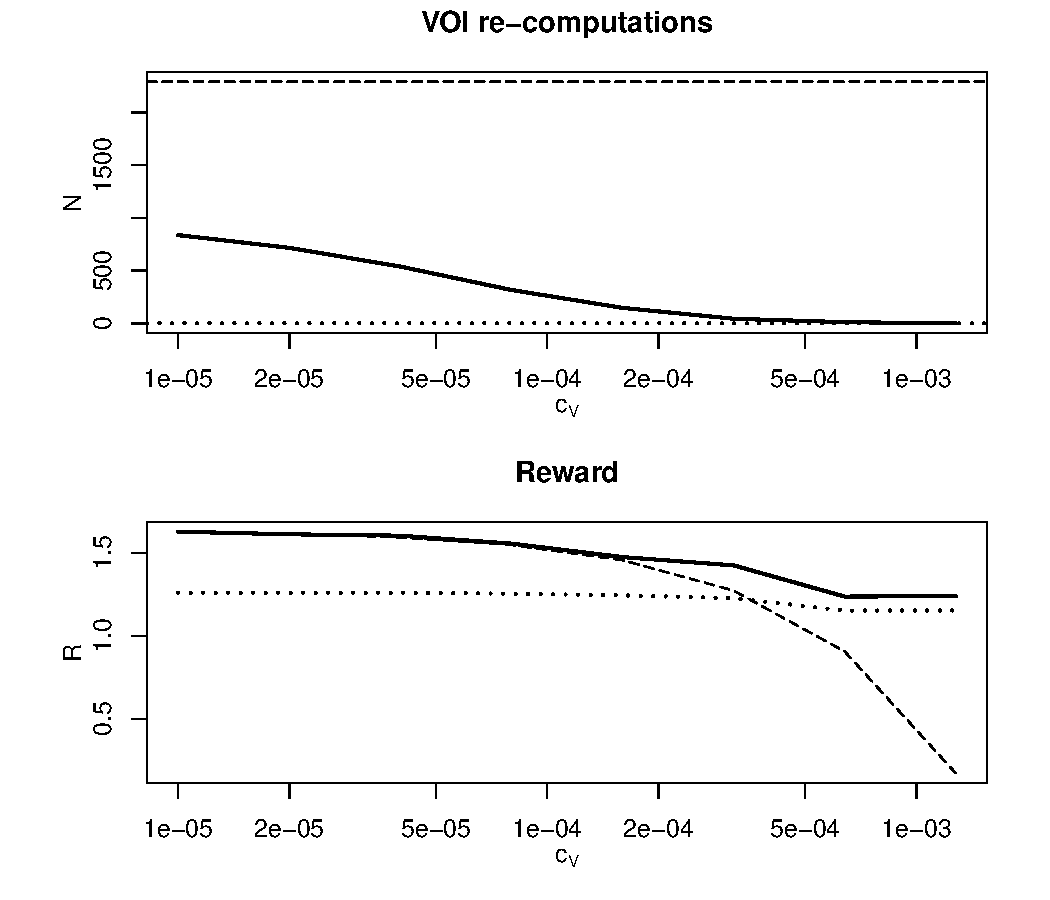
\includegraphics[scale=0.63]{raticomp-ackley.pdf}
\caption{The Ackley function.}
\label{fig:ackley}
\end{figure}
The Ackley function \cite{Ackley.function} is a popular optimization
benchmark. The two-argument form of the Ackley function is used in the
experiment; the function is defined by the expression (\ref{eq:emp-ackley}):
\begin{equation}
\label{eq:emp-ackley}
A(x,y)=20\cdot \exp\left(-0.2\sqrt { \frac {x^2+y^2} 2}\right)+\exp\left(\frac{cos(2\pi x)+cos(2\pi y)} 2\right)
\end{equation}
In the optimization problem, the utility function is
$u(z)=\tanh(2z)$, the measurements are normally distributed around the
true values with variance $\sigma_m^2=0.5$, and the measurement cost is
$0.01$. There are uniform dependencies with $\sigma_w^2=0.5$ in both
directions of the coordinate grid with a step of $0.2$ along each axis.
The results are presented in Figure~\ref{fig:ackley}.

\subsection{SVM Parameter Search}
\label{sec:raticomp-svm}

\begin{figure}[h]
\centering
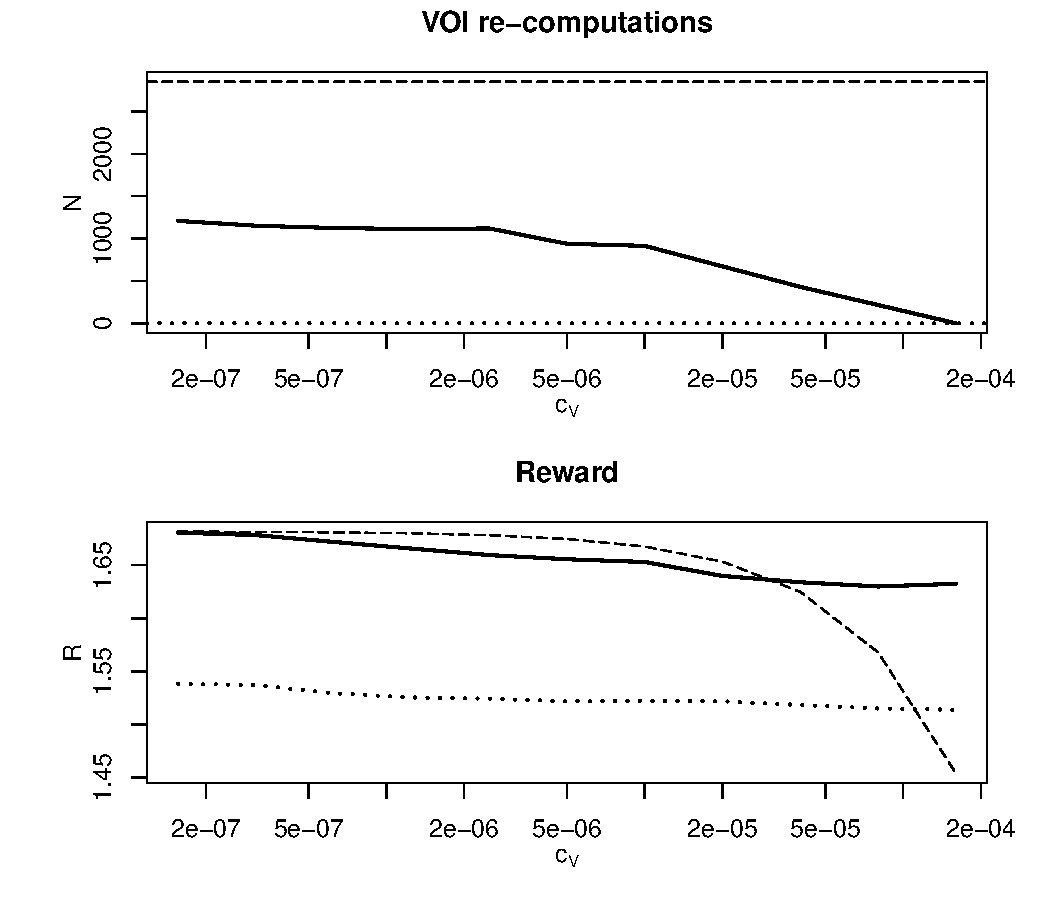
\includegraphics[scale=0.63]{raticomp-svmguide2.pdf}
\caption{SVM parameter search.}
\label{fig:svmguide2}
\end{figure}
An SVM (Support Vector Machine) classifier based on the radial basis
function has two parameters: $C$ and $\gamma$.  A combination of $C$
and $\gamma$ with high expected classification accuracy should be
chosen, and an efficient algorithm for determining the optimal values
is not known. A trial for a combination of parameters determines
estimated accuracy of the classifier through cross-validation. The
{\sc svmguide2} \cite{Hsu.dataset} dataset is used for the case study.
The utility function is $u(z)=\tanh(4(z-0.5))$, the $\log C$ and $\log
\gamma$ axes are scaled for uniformity to ranges $[1..21]$ and there
are uniform dependencies along both axes with $\sigma_w^2=0.4$. The
measurements are normally distributed with variance $\sigma_m^2=0.25$
around the true values, and the measurement cost is $c=0.01$.
The results are presented in Figure~\ref{fig:svmguide2}.

\subsection{Discussion of Results}

In all experiments, the reward, including the computation cost, of the
rational recomputing algorithm is comparable to or higher than the
reward of the original algorithm. When the computation cost is
relatively small (left-hand side of the plots), the rewards of the
rational recomputing algorithm and of the original algorithms are
essentially the same, despite the fact that much fewer VOI estimations are
computed. This suggests that the \textit{benefit of estimating the VOI}
of a measurement is in many cases low, and rational elective VOI
estimation is a viable approach to decreasing computation costs.
When the computation cost of VOI estimation grows, the rewards still
remain comparable, with the reward of the original algorithm only
slighter greater for the SVM parameter search
(Figure~\ref{fig:svmguide2}): a lower utility of the final choice of the
rational recomputing algorithm is compensated by a lower computation
cost. 

The advantage of the rational recomputing algorithm becomes obvious
when the cost of estimating the VOI of all measurements is comparable
to or exceeds the cost of performing a measurement (the right-hand side of
the plots). The reward of the original algorithm decreases rapidly,
falling below the reward of the Monte-Carlo algorithm. Rational
recomputing algorithm still performs well: the reward degrades
gradually with the increase of the computation cost, and approaches
asymptotically from above to the reward of random sampling (the
Monte-Carlo algorithm). 

Overall, the rational recomputing algorithm is robust, despite the
simplicity of the model. Both the case of a negligibly low computation
cost of VOI estimation, where both the original and the rational
recomputing algorithm exhibit good performance, and the case when the
cost of recomputation of VOI for all measurements is comparable to the
cost of performing a measurement are handled well: the reward is
almost as high as that of the original algorithm in the former case, and is
higher than that of Monte-Carlo algorithm performing the same number of
measurements in the latter case.

\section{Conclusion and Further Research}
\label{sec:raticomp-conclusion}

This chapter proposes an improvement to a widely used class of VOI-based
optimization algorithms. The improvement allows to decrease the
computation time while only slightly affecting the reward. The
proposed algorithm rationally reuses computations of VOI estimates and
recomputes the estimates only for measurements for which a change in
the VOI is likely to affect the choice of the next
measurement.

The proposed scheme of rational VOI computation can be further
improved. 
\begin{itemize}
\item  the normal distribution is chosen rather arbitrarily to model
  uncertainty about the VOI. Often, the VOI of a
  computational action decreases when other computational actions are  
  performed \cite{Guestrin.submodular}, and a skewed distribution from the
  exponential family should be chosen for better results.
\item The termination condition of VOI recomputation should be
  improved such that the VOI recomputation cost could be accounted for
  in the final reward.
\item The scheme is applied to the greedy algorithm
  for measurement selection, but can be extended to other
  VOI-based algorithms.
\end{itemize}


\chapter{Applications}
\label{ch:applications}

\section{Parameter Tuning}
\label{sec:app-apt}
Performance of heuristic algorithms and processes often depends on a
set of parameters. The parameters allow to optimize an algorithm for a
certain class of problems or to adapt a process to a particular
environment \cite{Leyton.paramils}. For example, classification
quality of a kernel-based classifier varies significantly depending on
kernel parameters; high-performance SAT solvers often have a number of
parameters, and must be tuned for a particular class of problems
\cite{Hutter.sat}. Thus, the optimization of algorithm performance by
automatically identifying good parameter settings is an important
problem, and a number of solution methods have been recently developed
\cite{Hutter.spo}. In general, the goal of the optimization problem is
to find, given a parameterized algorithm $\mathcal{A}$ and its utility
$u(\mathcal{A}, p)$ on a problem instance $p$, parameter settings for
$\mathcal{A}$ that maximize the expected utility $\IE_{p\in
\mathcal{P}}(u(\mathcal(A),p)$ over a set of problem instances
$\mathcal{P}$.

\subsection{Parameter Optimization as Selection Problem}

The parameter optimization problem can be viewed as a selection
problem \cite{TolpinShimony.blinkered} and solved using a
complete-state search:
\begin{itemize}
\item The state is a parameter assignment.
\item The utility of a state is the expected utility of $\mathcal{A}$
  on the problem set $\mathcal{P}$. 
\item A computational action estimates the expected utility of
  $\mathcal{A}$ by running $\mathcal{A}$ on a subset of $\mathcal{P}$.
\end{itemize}
Observe that the computational action provides a noisy utility
estimate both because $\mathcal{A}$ can be randomized, and because
$\mathcal{A}$ is applied only to a subset of the problems.

\subsubsection{Examples}

In the problem of tuning parameters for an {\bf SVM classifier}
based on RBF kernel \cite{TolpinShimony.blinkered}, the parameters are
the kernel curvature $\gamma$ and the misclassification cost $C$. The
parameters are selected based on a training set for a particular
problem domain. The classifier with the chosen parameters is then used
for classification of samples in the domain.

{\bf Mixed integer programming solvers} are highly parameterized
\cite{Hutter.mip}. Their parameters control a wide range of design
choices on preprocessing techniques, branching and cutting heuristics,
details of the underlying linear programming solver. Robust default
parameter settings can sometimes be identified, but an algorithm tuned
for a particular family of problem instance can significantly
outperform the default configuration.

\subsection{Solution techniques}

The basic metareasoning algorithm used to solve the selection problem
selects computational actions according to the myopic estimate
\cite{Russell.right} and generally works well. However, the
simplifying assumptions behind the myopic estimate are related to the
notion of {\it non-increasing returns}: an implicit hypothesis that
the intrinsic value of information grows slower than the cost. When
the hypothesis is incorrect, the estimate performance can be
poor. Semi-myopic estimates improve the algorithm performance and be
used to solve problems with noisy utility estimates, such as in the
case of assessing the algorithm performance based on a small subset of
the problem set \cite{TolpinShimony.blinkered}.

However, the metareasoning algorithm still requires rather tight
parameter ranges containing the optimal combination of values, and
only works well for a relatively small number of parameters.  In some
cases, feasible ranges of parameter values can be guessed, and the
most influential parameters can be identified through
pre-processing. In the general case, however, algorithms that can
handle large and high dimensional parameter spaces are important.

\subsection{Future research}
\label{sec:app-apt-research}

{\bf Large} or {\bf infinite parameter space} requires an algorithm
that bounds the set of simultaneously available computational actions
(Section~\ref{sec:raticomp-infinite-spaces}). Such algorithm would
alleviate the need to heuristically guess default or initial parameter
values before the search, as is currently done, for example, for the
SVM classifier, and, at the same time, determine a good parameter
assignment with greater accuracy.

{\bf High dimensional parameter spaces} are challenging because
the number of computational actions is proportional to the size of the
parameter product domain. One technique is applicable when the evaluation
of a single combination of parameters is cheap, and dependencies
between parameters are hierarchical. In such a case, a semi-sequential
parameter optimization can be used: the most
influential parameters at the top of the hierarchy can be determined
using a metareasoning search, and each computational action determines
the best combination of a subset of parameters belonging to a subtree
using a simpler technique such as sequential parameter optimization or
even uninformed search. 

Initial results in this direction were obtained for optimization
of thresholds in a rule-based classifier.  The rule tree had 10
optimization parameters. Three parameters were heuristically chosen
for optimization using a rational search algorithm, values for the remaining
seven parameters were chosen using a simple search algorithm
(iterative sequential optimization). The new parameter values improved
accuracy of the classifier, already optimized using a different
optimization method, from 0.948 to 0.969.

\section{Counting~Based Heuristics for~Constraint~Satisfaction}
\label{sec:app-csp}
Performance of backtracking search
(Section~\ref{sec:bg-backtracking-search}) for constraint satisfaction
problems is strongly influenced by the quality of heuristics
\cite{Tsang.csp}. There are both domain-specific heuristics, helpful
in solving a particular class of problems, such as heuristics for SAT
solvers \cite{Krautz.sat}, and domain independent heuristics,
applicable to a wide range of problems, such asvariable and value
ordering heuristics based on characteristics of the constraint graph
\cite{Tsang.csp}.

Sophisticated heuristics are computationally intensive, and the effect
of an heuristic may or may not justify the computation time
\cite{Refalo.impact}. Heuristic parameters are introduced to control
selective or adaptive application of heuristics
\cite{Wallace.macheur}.

The metareasoning layer can control adaptive application
of certain CSP heuristics. One such heuristic is the {\em solution counting}
heuristic for value ordering \cite{Kask.solcount}. 

\subsection{Constraint satisfaction problem}

A constraint satisfaction problem (CSP) is defined by a set
of variables, $X_1$, $X_2$, ..., $X_n$, and a set of constraints,
$C_1$, $C_2$, ..., $C_n$. Each variable $X_i$ has a non-empty domain
$D_i$ of possible values. Each constraint $C_i$ involves some subset
of the variables---the scope of the constraint--- and specifies the
allowable combinations of values for that subset. An assignment that
does not violate any constraints is called a consistent assignment.

A constraint satisfaction problem may or may not have a consistent
assignment. A problem instance is called consistent if there is a
consistent assignment, and inconsistent otherwise. In this section,
the satisfaction problem of finding a consistent assignment or proving
that no such assignment exists is considered. Graph coloring
and sudoku puzzle are examples of such problems.

The performance of a search algorithm for the CSP problem is
determined by the computation time required to either find a
consistent assignment or to prove that the problem is inconsistent. In
general, the CSP problem is NP-hard (by reduction from 3SAT), but many
instances are actually solvable in polynomial time with the help of
appropriate heuristics.

\subsection{Maintaining arc consistency}

The basic algorithm on top of which many heuristic algorithms are
built is the MAC (Maintaining Arc Consistency) algorithm
\cite{Sabin.mac}. There are several versions of MAC. The versions
differ in efficiency, but share the common feature of maintaining {\em
arc consistency}, defined for CSP problems with binary constraints. A
variable $X_i$ is arc-consistent with $X_j$ if for every value $a$ of
$X_i$ from the domain $D_i$ there is a value $b$ of $X_j$ from the
domain $D_j$ satisfying the constraing between $X_i$ and $X_j$. MAC
maintains arc constistency for all pairs of variables.

Arc consistency is implemented in the function {PropagateConstraints}
of Algorithm~\ref{alg:bg-backtracking-search} of
Section~\ref{sec:bg-backtracking-search}.  A pseudocode for MAC-3
\cite{Russell.aima} is presented in Algorithm~\ref{alg:app-csp-mac-3}.
\begin{algorithm}
\caption{Maintaining Arc Consistency}
\label{alg:app-csp-mac-3}
\begin{algorithmic}[1]
\item[{\bf MAC-3}$(csp):$]
\STATE $queue \leftarrow$ all arcs in $csp$
\WHILE {$queue$ not empty}
  \STATE $(X_i, X_J) \leftarrow RemoveFirst(queue)$
  \IF {$RemoveInconsistentValues(X_i, X_j)$}
    \FORALL {$X_k$ {\bf in} $Neighbors(X_i)$}
      \STATE $Add(queue, (X_k, X_i))$
    \ENDFOR
  \ENDIF
\ENDWHILE
\vspace{1em}
\item[${\bf RemoveInconsistentValues}(X_i, X_j)$]
  \STATE $removed \leftarrow {\bf false}$
  \FORALL {$x$ {\bf in} $D_i$}
    \IF {no value $y$ in $D_j$ allows $(x, y)$}
        \STATE $D_i \leftarrow D_i \setminus \{x\}$
        \STATE $removed \leftarrow {\bf true}$
    \ENDIF
  \ENDFOR
  \RETURN {$removed$}
\end{algorithmic}
\end{algorithm}
MAC speeds up the backtracking search by pruning many inconsistent
branches. However, the variable and value ordering heuristics
significantly improve the algorithm performance. Many such heuristics,
based on the variable domain, degree \cite{Sabin.mac}, impact of the
value assignment \cite{Refalo.impact} etc, are known.

\subsection{Counting-based value-ordering}

A powerful value-ordering heuristic is based on solution counting
\cite{Meisels.solcount}: solution counts for each value
assignment of the current variable are estimated, and an assignment
with the greatest solution count is selected. The heuristic is based
on the assumptions that sizes of the subtrees for each of the
assignment do not vary too much, and thus the more solutions there are
in the subtree, the shorter the time to arrive at the first solution.
Experiments show that the heuristic indeed significantly improves the
search performance for a range of problem domains
\cite{Meisels.solcount}\cite{Kask.solcount}.

Computing the exact number of solutions is \#P-hard (because CSP is
NP-hard), but there are several ways to estimate the solution count:
\begin{itemize}
  \item Meisels, Shimony and Solotorevsky \cite{Meisels.solcount}
        reduce solution counting to computing marginal probabilities in a
        Bayesian network equivalent to the constraint graph.
  \item Kask, Dechter and Gogate \cite{Kask.solcount} use Iterative
        Joint Graph Propagation adapted for solution counting.
  \item Gomes, Hoeve et al. \cite{Gomes.solcount} propose a technique
        that adds random generalized XOR constraints and counts solutions with
        high precision.
\end{itemize}
The methods vary by the computation time and precision, and a
thorough comparative study should be conducted to choose the best
implementation of the heuristic. However, application of principles of
rational metareasoning is independent of the implementation choice.

\subsection{Rational application of the heuristic}
\label{sec:app-csp-rational}

Solution counting is computationally intensive, and empirical evaluation
\cite{Kask.solcount} demonstrates that while in general the heuristic
improves the algorithm performance, for certain problem sizes it is
better to order values arbitrarily instead of computing the heuristic.

A rational agent can apply the heuristic sequentially, one assignment
at a time. When the expected speedup is less than the time to estimate
the solution count, the agent chooses a value ordering and commits to
an assignment. It remains to determine how the solution count and the
time to a solution are interrelated.

To estimate the VOI, a simplified model of the value ordering must be
devised.
\begin{enumerate}
\item Subproblem sizes corresponding to all value assignments to a
   given variable are assumed equal: the expected time to find a solution
   depends only on the solution count. This assumption can be lifted
   later, by combining solution counting with an impact-based
   heuristic \cite{Refalo.impact}. Experiments conducted in prior work
   \cite{Meisels.solcount}\cite{Kask.solcount} demonstrate that
   ignoring the differences in subproblem sizes is justified.
\item Solutions are assumed to be evenly distributed in the search
  space, that is, the time to find a solution is distributed as the
  time between events in the Poisson process.
\item The solution count estimate is the mean number of solutions
  in the subproblem. The number of solutions is distributed according
  to the Poisson distribution.
\end{enumerate}
In the above assumptions, distributions are used in the Bayesian
sense and denote beliefs rather than frequencies. 

Consider first the hypothetical case when solution counts are computed
exactly. Let $N$ be the number of solutions in the tree, and the mean
time to find all of the solutions is $T$. Then, knowing the number of
solutions $n$ for a particular assignment of value $y$ to variable $X$
with domain $D$ may improve the expected time to the first solution in
one of the following two ways:
\begin{itemize}
\item Either $\frac T {|D|n} < \frac T N$, and then the time gets shorter by $T \left( \frac 1 N - \frac 1 {|D|n}\right)$. 
\item Or $\frac T {|D|n} > \frac T N$, but then $\frac {T(|D|-1)} {|D|(N-n)} < \frac T N$, and the time gets shorter by $T \left( \frac 1 N - \frac {|D|-1} {|D|(N-n)}\right)$.
\end{itemize}

Continuing recursively, if the currently highest solution count
$n_\alpha$ is achieved for some assignment $X=y_a$, then the
improvement due to counting solutions for another assignment is:
\begin{itemize}
\item Either $\frac T {|D|} \left( \frac 1 {n_\alpha} - \frac 1 n\right)$ if $n > n_\alpha$.
\item Or $\frac T {|D|} \left (\frac 1 {n_\alpha} - \frac {|D'|-1} {N'-n} \right)$ if $\frac {N'-n} {|D'|-1} > n_\alpha$.
\end{itemize}
where $D'$ is the set of assignments for which the solution count was
not estimated, and $N'$ is the total number of solutions corresponding
to the assignments, computed as the total number of solutions $N$ less
the sum of the computed solution counts: $N'=N-\sum_{y \in D\setminus D'} SC(y)$.
Unless $|D'|\approx 1$, the latter case is significantly less
influential than the former and can be ignored for simplicity.

When only the {\em mean values of beliefs} about the number of solutions are
known, the computation becomes more involved: the assignment with the
highest mean solution count $\nu_{\alpha}$ can actually lead, with the
corresponding probability, to any number of solutions, including no
solutions. The search backtracks with probability
$p_0=e^{-\nu_{\alpha}}$ from the assignment and continues to other
assignments. However, efficiency in estimating VOI is more important
than accuracy, and the probability of no solutions
decreases rapidly with the mean number of solutions $\nu$, $\approx 0.14$ for
$\nu=2$, $\approx 0.007$ for $\nu=5$, $\approx 0.00005$ for $\nu=10$
and so on. Consequently, for the purpose of estimating the VOI the
event of backtracking from the assignment can be ignored, and the
{\em benefit} (intrinsic value of information) of computing the number of
solutions of an assignment can thus be estimated as follows:
\begin{equation}
\label{eq:app-csp-lambda-simplified}
\Lambda = \frac T {|D|} \sum_{n_\alpha=1}^\infty\left[\sum_{n=n_\alpha}^\infty \left( \frac 1 {n_\alpha} - \frac 1 n\right) p_\nu(n)\right]p_{\nu_{\alpha}}(n_\alpha)
\end{equation}
Further on, the outer summation by can be approximated by setting $n_\alpha=\nu_\alpha$:
\begin{equation}
\label{eq:app-csp-lambda-simple}
\Lambda= \frac T {|D|} \sum_{n=\nu_\alpha}^\infty \left( \frac 1 {\nu_\alpha} - \frac 1 n\right) p_\nu(n)
\end{equation}
where $\nu=\frac {N'} {|D'|}$ -- solution rate per assignment, and
$p_\nu(n)=\frac {e^{-\nu}\nu^n} {n!}$ is the probability to find $n$
solutions when the mean number of solutions is  $\nu$.

Estimating solution counts makes sense only if the expected improvement in the
running time ($\Lambda$) is greater than the time $T_c$ spent
estimating the solution count. While $T_c$ can be estimated for a
particular implementation of solution counting, $T$ in the equation
for the benefit is still unknown and {\em depends on application of
the heuristic}. However, it is reasonable to assume that counting
solutions is somewhat similar to finding solutions, and that $T_c$ is
proportional to $T$ with an unknown factor $\gamma < 1$.
\begin{equation}
\label{eq:app-csp-gamma}
T_c = \gamma T
\end{equation}
Then, $T$ can be eliminated from both $T_c$ and $\Lambda$. Solutions
are counted when
\begin{equation}
\label{eq:app-csp-solcount-condition}
\sum_{n=\nu_\alpha}^\infty \left( \frac 1 {\nu_\alpha} - \frac 1 {n}\right) \frac {\nu^n} {n!} > {|D|}e^\nu \gamma
\end{equation}
and $\gamma$ can be learned offline from a set of problem instances of a certain kind
for the given implementation of the search algorithm and the solution
counting heuristic. While there is still a parameter that must be
learned empirically, the decision whether to apply the heuristic is
based on a solid foundation of the decision theory.

Algorithm~\ref{alg:app-csp-solcount} implements the value ordering heuristics based on solution counting.
\begin{algorithm}
\caption{Value Ordering via Solution Counting}
\label{alg:app-csp-solcount}
\begin{algorithmic}[1]
\item[{\bf ValueOrdering-SC}$(csp, X)$]
\STATE compute the total mean solution count: $N \leftarrow SolutionCount(csp)$
\STATE retrieve the domain of $X$: $D \leftarrow Domain(X)$
\STATE initialize the highest mean solution count: $\nu_\alpha \leftarrow \frac N {|D|}$
\FORALL {$y$ {\bf in} $Domain(X)$}
  \STATE initialize solution count for assignment: $\nu(y) \leftarrow \nu_\alpha$
\ENDFOR

\WHILE {$VOI(nu_\alpha)>0$}
  \STATE choose $y \in D$ arbitrarily
  \STATE remove $y$ from the domain $D$: $D \leftarrow D \ \{y\}$
  \STATE restrict the domain of $x$ in $csp$ to a single value: $csp' \leftarrow CSP|Domain(x)=\{y\}$
  \STATE count solutions in $CSP'$: $\nu(y) \leftarrow SC(CSP')$
  \STATE decrease the remaining solution count by $\nu(y)$: $N \leftarrow N - \nu(y)$
  \STATE update solution count for all uncounted values to: $N/|D|$
  \IF {$\nu(y) > \nu_\alpha$}
    \STATE update the highest count: $\nu_\alpha \leftarrow \nu(y)$
  \ENDIF
  \ENDWHILE
\RETURN $Domain(X)$ in the decreasing order of $nu(y)$
\end{algorithmic}
\end{algorithm}

Initial experiments on Sudoku and random CSP instances show that the
amount on computation can be flexibly controlled by changing the value
of $\gamma$.

\subsection{Future research}

Theoretical analysis of the solution counting heuristic must be
completed. In particular, a VOI estimate that accounts for the
probability of backtracking and the distribution of solution counts
for the currently best assignment must be compared with the simplified
estimate, theoretically and empirically. Optimally, an estimate that
combines simplicity and provable approximation bounds should be
derived.
 
Except for the early encouraging results on relatively small problem
instances, empirical evaluation of the algorithm with rational
heuristic application has not been conducted yet and is required to
assess the improvement in performance and robustness. Different
algorithms for solution counting must be compared, and the most
appropriate algorithm should be chosen for implementation of the
heuristic. 

Solution counting for value ordering is just one heuristic among the
many used to solve CSP problems. In particular, there are
heuristics, such as the impact-based heuristic proposed by
Refalo \cite{Refalo.impact}, which are based on the assumption that
the CSP instance is inconsistent, and the whole tree will have to be
traversed or pruned to prove the inconsistency. Rationally choosing between
heuristics working better for either consistent or inconsistent
problem instances, in addition to rational selective application of
heuristics within each group, may further improve the search
performance. 


\section{Remote~Sensing in Canadian~Traveller Problem}
\label{sec:app-ctp}
In the {\em Canadian Traveler Problem} (CTP) \cite{Barnoy.ctp} a
traveling agent is given an undirected connected weighted graph
$G=(V,E)$ as input together with its initial source vertex ($s \in
V$), and a target vertex ($t \in V$).  The input graph $G$ may undergo
changes, that are not known to the agent, {\em before} the agent
begins to act, but remains fixed subsequently.  In particular, some of
the edges in $E$ may become {\em blocked} and thus untraversable. Each
edge $e$ in $G$ has a weight, or cost, $w(e)$, and is blocked with a
probability $p(e)$, where $p(e)$ is known to the agent. The agent can
perform {\em move} actions along an unblocked edge which incur a {\em
  travel cost} $w(e)$.  Traditionally, the CTP was defined such that
the status of an edge can only be revealed upon arriving at a node
incident to that edge, i.e., only {\em local sensing} is allowed.

A somewhat more general version of CTP is {\em CTP with sensing}. In
this variant, in addition to move actions (and local sensing), an
agent situated at a vertex $v$ can also perform {\em sense} actions
and query the status of any edge $e \in G$. The sensing action incurs a
{\em sensing cost} $sc(v,e)$. The task of the agent is to travel to
the goal while minimizing a total cost
$C_{total}=C_{travel}+C_{sensing}$.

In a general case, value of information of a sensing action can be
efficiently estimated only under rather strong simplifying
assumptions, such as the free-space assumption
\cite{Bnaya.sensing}. Special cases in which a better VOI estimate can
be computed efficiently are of interest.

In one such setting, the sensing costs are much smaller than the
travel costs, and it makes sense to ensure that the path to be
traversed is open before beginning traversal.  In this variant, called
{\em CTP-Sensing-First} (CTP-SF), the problem is to minimize expected
sensing costs in order to detect the shortest open path. The
base-level action uses a polynomial-time algorithm (such as the
Dijkstra algorithm for the single-source shortest path problem
\cite{Kleinberg.algorithms}) to find the shortest path between the
source and the target nodes.

\subsection{Proposed research}
\label{sec:app-ctp-research}

An algorithm based on rational
metareasoning can be used to solve the CTP-SF problem, which can be
formulated as follows:
\begin{itemize}
\item The application of a polynomial-time CTP algorithm to the CTP
  graph updated according to the remote sensing outcomes is the only
  base-level action.
\item The travel cost of the algorithm, taken with the negative sign,
  corresponds to the utility of the base-level action.
\item The remote sensing actions, performed before the traditional CTP
  algorithm is applied, correspond to the computational actions.
\end{itemize}
This problem can be solved approximately using weaker simplifying
assumptions than for the general case of CTP with sensing, since the
sensing and the traversal are not interleaved, and the net utility of
the base-level action is easily computable. Optimal solutions for
restricted cases of the problem with particular graph topology may be
discovered. Finally, the algorithm for solving the CTP-SF problem
can be used to design an heuristic for solving the general CTP problem
with sensing.

\section{Learning Bayesian Networks from Large Datasets}
\label{sec:app-bnlearn}
Bayesian network is a formalism for describing causal dependencies
between variables \cite{Pearl.PRIS}. Bayesian networks are widely used
for encoding domain knowledge, both provided by experts and learned
from data.  Bayesian networks facilitate combining expert and learned
knowledge complementing each other.

\subsection{Motivation for learning Bayesian network structure}

A Bayesian network is a pair $B=(G, \Theta)$ where $G=(V,E)$ is a directed
graph and $\Theta$ are are numerical vertix labels
\cite{Heckerman.tutorial}. Vertices of the graph $V$ correspond to variables,
the edges $E$ denote causal relations between the variables, and the labels
quantify the relations. Bayesian networks are used for {\it
inference}: given a {\it prior belief} and an {\it evidence} for a
Bayesian network, the posterior distribution of variable values can be
computed.

In some cases, the initial structure of a Bayesian network can be
provided by an expert, in other cases the structure is unknown and
has to be discovered. In either case, training data can be used
to learn or improve the Bayesian network, both the structure and the
parameters. However, learning Bayesian networks is NP-hard 
\cite{Chickering.learningbayesian}, therefore heuristic-based
approximate algorithms are used \cite{Heckerman.tutorial}.

\subsection{Approaches to Bayesian network learning}

Two widely adopted approaches to learning Bayesian networks are {\it
  score-based} and {\it constraint-based}. In the score-based
approach, a score is assigned to each Bayesian network and reflects
how well the network describes the data set. Then, a network with
the highest score is selected from a candidate set. In the
constraint-based approach, conditional independence tests are
performed on variables, and a network satisfying the discovered
conditional independence properties is built. 

Algorithms adhering to the score-based approach are based on 
such heuristic search techniques as greedy hill-climbing or
simulated annealing \cite{Heckerman.tutorial}. Constraint-based
algorithms use heuristics to discover conditional independence
relations between variables, and then infer the graph structure; since
an exponential number of tests is required to discover the relations,
domain knowledge and heuristics are used to performs tests selectively
and build an approximate solution.

When the data set used to learn the structure is large, even
polynomially bounded approximate algorithms require enormous time. One
approach for learning Bayesian network structure from large data sets
is the ``Sparse candidate algorithm'' which selectively uses
conditional independence tests to direct score-based
search \cite{Friedman.sparsecandidate}. The Bayesian network can itself
be large and consist of hunderds of thousands of nodes. Such network
has to be learned from a large sparse data set; and Goldenberg and Moore
\cite{Goldenberg.sparsedata} describe a score-based algorithm which uses
``Frequent Sets''---sets of attributes which occur frequently in the
sparse data---as the heuristic. Other authors also use various
heuristics to deal with vast amounts of data and long computation
times (\cite{Zhou.clustering}, \cite{Boyen.hidden}).

\subsection{Proposed research}
\label{sec:app-bnlearn-research}

The time to compute heuristics can be significant. Selective
application of heuristics justified by the anticipated benefit should
improve the running times and make the algorithms applicable to large
problem instances. In particular, the mentioned score-based approach
can be cast as a complete-state search problem in a large search
space. To improve the performance of score-based learning,
a rational metareasoning algorithm should be used to search for
the Bayesian network structure. An appropriate dependency model for
candidate networks must be chosen, and a proper estimate for the
utility of structure scoring must be invented for such algoirthm. 

Computing the score of a candidate is expensive for large data sets. A
rational metareasoning algorithm should be used for approximate score
evaluation. This is especially relevant if a structure currently under
consideration can be quickly ruled out as a candidate based on a rough
score estimation, compared to another structure already scored by the
algorithm.  The approximate scoring algorithm would select for
computing the score a subset of the data set with the highest value of
information estimate. Both online and offline subset selection
algorithms \cite{Guestrin.graphical} should be considered.

Since the search spaces of structure candidates and of data instances
are large, the algorithms would also use the research results for
large search spaces (Section~\ref{sec:raticomp-infinite-spaces}).



\chapter {Summary and Expected Contribution}
\label{ch:summary}
The thesis comprises two major topics:
\begin {enumerate}
\item Rational computation of value of information (Chapter~\ref{ch:raticomp}).
\item Case studies of application of rational metareasoning to
  selection and application of heuristic computations (Chapter~\ref{ch:case-studies}).
\end {enumerate}

The first topic addressed cases in which estimating the value
of information of a computational action is expensive, as well as
cases of too many computational actions, such that although
estimating the value of information of a single action is cheap,
estimating the value of information of all actions at each step of the
algorithm is expensive. The research, published in
\cite{TolpinShimony.raticomp}, resulted in an improvement to a widely
used class of VOI-based optimization algorithms that allows to decrease the
computation time while only slightly affecting the reward. Theoretical
analysis of the proposed approach to rational computation of the
value of information was supported by empirical evaluation of several
combinations of algorithms and search problems.

The second topic considered several search problems and improved some
well-known algorithms for solving the problems using the rational
metareasoning approach:
\begin {itemize}
\item Adaptive deployment of value-ordering heuristics in constraint
  satisfaction problems (Section~\ref{sec:cs-csp}) \cite{TolpinShimony.csp};
\item Monte Carlo tree search based on simple regret
  (Section~\ref{sec:cs-mcts}) \cite{TolpinShimony.mcts,HayRussellTolpinShimony.selecting};
\item Decreasing heuristic evaluation time in a variant of A*
  (Section~\ref{sec:cs-rla}) \cite{TolpinEtAl.rla}. 
\end {itemize}
In addition to the algorithm improvements, the studies demonstrated a
number of common rational metareasoning techniques which can be 
extended to other problem types. In particular,
\begin{itemize}
\item Section~\ref{sec:cs-mcts}, ``VOI-aware Monte-Carlo tree search''
provided distribution-independent upper bounds for semi-myopic VOI
estimates in Monte-Carlo sampling.
\item Section~\ref{sec:cs-rla}, ``Towards rational deployment of Multiple
Heuristics in A*'', introduced a novel area of application of rational
metareasoning---optimal search in optimization problems.
\end{itemize}

As a whole, the research advanced the use of rational
metareasoning in problem-solving search algorithms. Applications of
rational metareasoning in the case studies serve as examples
to help researchers employ the methodology in solutions for other
problems. Advances in rational computation and estimation of VOI increase
performance and applicability of existing and new search algorithms
and alleviate dependence of algorithm performance on manual
fine-tuning.

The field of rational metareasoning still poses serious
challenges. An important yet unanswered question is the extent
to which algorithm performance can be improved due to employment of
the metareasoning approach. In the case studies presented in the thesis,
the improvements, while approached the theoretical limits of each
particular algorithm variant, were moderate. It is still not clearly
understood \textbf{whether a dramatic breakthrough in performance is possible}
if more elaborated models of utility and information are used, or the 
limitations are immanent to the approach itself. Another interesting
field of research is rational metareasoning where \textbf{action costs and
state utilities are not commensurable}. Instead of mapping between
different measures, as suggested in Chapter~\ref{ch:raticomp}, a
more general combination function should probably be used for best
results. Ways of choosing or deriving such a function still remain
to be discovered.


\bibliographystyle{alpha}
\bibliography{refs}

\end{document}
